%initialising document, adjust papersize, fontsize and page orientation to your needs
\documentclass[a4paper, fontsize = 8pt, landscape]{scrartcl}
\usepackage{../../../misc_files/LateX/layout_and_colours}
\title{Computertechnik}
\author{Jil Zerndt, Lucien Perret}
\date{May 2024}

\createtitlepagestyle
\createmainpagestyle
\begin{document}
\begin{multicols}{3}
	\thispagestyle{TitlePageStyle}
	\maketitle

	\section{Computer Engineering}

\begin{concept}{Computer Engineering}
is where microelectronics and software meet:
\begin{itemize}
  \item Architecture and organization of computer systems
  \item Combines hardware and software to implement a computer
  \item Applications in embedded systems, information technology, and technical/scientific tools
  \item Historical development spanning over 70 years:
    \begin{itemize}
      \item 1940s: Relay/vacuum tubes
      \item 1950s: Transistors
      \item 1970s: Integrated circuits (CMOS)
      \item Present: Complex microprocessors with billions of transistors
    \end{itemize}
\end{itemize}
\end{concept}

\begin{theorem}{von Neumann Architecture}\\
The fundamental architecture used in most computers:
\begin{itemize}
  \item Single memory for both data and instructions
  \item Sequential instruction execution
  \item Components: Control unit, ALU, memory, Input/Output
  \item Key limitation: Memory bottleneck ("von Neumann bottleneck")
\end{itemize}
\end{theorem}

\subsubsection{Hardware}

\begin{definition}{Basic Hardware Components}\\
A computer system consists of four fundamental components:
\begin{itemize}
  \item \textcolor{cornflower}{\textbf{CPU (Central Processing Unit)}}: Processes instructions and data
  \item \textcolor{frog}{\textbf{Memory}}: Stores instructions and data
  \item \textcolor{corn}{\textbf{Input/Output}}: Interface to external devices
  \item \textbf{System Bus}: Electrical connection between components 
    \begin{itemize}
      \item Address lines: Select memory location
      \item Data lines: Transfer data (8/16/32/64 bits)
      \item Control signals: Coordinate operations
    \end{itemize}
\end{itemize}

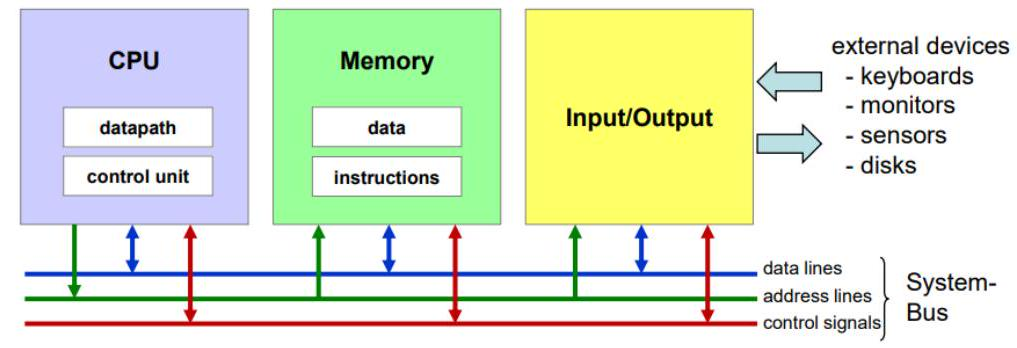
\includegraphics[width=\linewidth]{images/2024_12_29_79e6b22f503fb7b4f718g-01(1)}
\end{definition}

\begin{examplecode}{CPU Components}
The CPU contains several key components:

\textcolor{cornflower}{\textbf{Datapath:}}
\begin{itemize}
  \item \textbf{Core Registers}: Fast but limited storage inside CPU
  \item \textbf{ALU (Arithmetic Logic Unit)}: Performs arithmetic and logic operations
  \end{itemize}
\textcolor{cornflower}{\textbf{Control Unit}}: 
    \begin{itemize}
      \item Finite State Machine: Reads and executes instructions
      \item Controls program flow and manages instruction pipeline
    \end{itemize}
  \textcolor{cornflower}{\textbf{Bus Interface}}: Connects CPU to system bus
\end{examplecode}

\begin{corollary}{Memory} \\
A set of storage cells and the smallest addressable unit is a byte.

$2^N$ addresses:
\begin{itemize}
  \item RAM (Random Access Memory): read/write
  \item ROM (Read-Only Memory): read-only
\end{itemize}
\end{corollary}

\raggedcolumns




\begin{corollary}{Memory Types}
\begin{itemize}
  \item \textbf{Main Memory (Arbeitsspeicher)}:
    \begin{itemize}
      \item Connected through System-Bus
      \item Access to individual bytes
      \item Volatile: 
        \begin{itemize}
          \item SRAM (Static RAM) - faster, more expensive
          \item DRAM (Dynamic RAM) - needs refresh, cheaper
        \end{itemize}
      \item Non-volatile: 
        \begin{itemize}
          \item ROM - factory programmed
          \item Flash - in-system programmable
        \end{itemize}
    \end{itemize}
  \item \textbf{Secondary Storage}:
    \begin{itemize}
      \item Connected through I/O
      \item Access to blocks of data
      \item Non-volatile
      \item Examples: HDD, SSD, CD, DVD
      \item Slower but cheaper than main memory
    \end{itemize}
\end{itemize}
\end{corollary}

\begin{concept}{Memory Addressing}
\begin{itemize}
  \item Each byte in memory has a unique address
  \item Address space depends on address bus width:
    \begin{itemize}
      \item 8-bit address bus: 256 bytes ($2^8$)
      \item 16-bit address bus: 64 KB ($2^{16}$)
      \item 32-bit address bus: 4 GB ($2^{32}$)
    \end{itemize}
  \item Memory map shows allocation of address ranges
\end{itemize}
\end{concept}

\begin{KR}{Key concepts for working with memory}\\
1. Memory terms:
\begin{itemize}
  \item \textbf{Word}: A 32-bit memory unit
  \item \textbf{Half-word}: A 16-bit memory unit
  \item \textbf{Word Alignment}: Address is multiple of word size (4)
\end{itemize}

2. Endianness handling:
\begin{itemize}
  \item \textbf{Little endian}: LSByte at lower address
  \item \textbf{Big endian}: MSByte at lower address
\end{itemize}
\end{KR}

\begin{formula}{Program Translation Process} from C to executable
  \vspace{1mm}\\
Translation from source code to executable involves four steps:

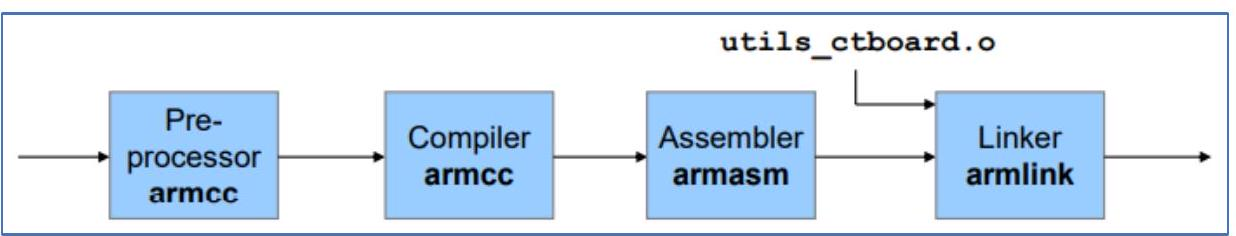
\includegraphics[width=\linewidth]{images/2024_12_29_79e6b22f503fb7b4f718g-01}

\begin{enumerate}
  \item \textbf{Preprocessor}: Text processing
    \begin{itemize}
      \item Includes header files (\#include)
      \item Expands macros (\#define)
      \item Output: Modified source program (.i)
    \end{itemize}
  \item \textbf{Compiler}: Translates C to assembly
    \begin{itemize}
      \item CPU-specific code generation
      \item Optimization (if enabled)
      \item Output: Assembly program (.s)
    \end{itemize}
  \item \textbf{Assembler}: Converts assembly to machine code
    \begin{itemize}
      \item Creates relocatable object file
      \item Generates symbol table
      \item Output: Binary object file (.o)
    \end{itemize}
  \item \textbf{Linker}: Merges object files into executable
    \begin{itemize}
      \item Resolves dependencies
      \item Relocates addresses
      \item Links with libraries
      \item Output: Executable file (.axf)
    \end{itemize}
\end{enumerate}
\end{formula}

\begin{KR}{Program Compilation Process}\\
To compile and link a program:
\begin{enumerate}
  \item Create source files (.c) and header files (.h)
  \item Run preprocessor to expand includes and macros
  \item Compile source files to object files
  \item Link object files and libraries
  \item Test executable
\end{enumerate}

Common compiler flags:
\begin{itemize}
  \item -c: Compile only, don't link
  \item -o: Specify output file name
  \item -O[0-3]: Optimization level
  \item -g: Include debug information
\end{itemize}
\end{KR}

\begin{code}{Simple Program Translation - From Source to Executable}
\begin{lstlisting}[language=C, style=basesmol]
// source.c
#include <stdio.h>
#define MAX 100

int main(void) {
    printf("Max is %d\n", MAX);
    return 0;
}
\end{lstlisting}

After preprocessing (.i):
\begin{lstlisting}[language=C, style=basesmol]
// Contents of stdio.h included here
int main(void) {
    printf("Max is %d\n", 100);
    return 0;
}
\end{lstlisting}

Assembly output (.s):
\begin{lstlisting}[language=armasm, style=basesmol]
    AREA |.text|, CODE, READONLY
    EXPORT main
main
    PUSH {LR}
    LDR R0, =string1
    LDR R1, =100
    BL printf
    MOVS R0, #0
    POP {PC}
    ALIGN
string1 DCB "Max is %d\n",0
    END
\end{lstlisting}
\end{code}

\begin{example2}{Host vs Target Development}\\
When developing for embedded systems:
\begin{itemize}
  \item \textbf{Host}: Development computer where code is written and compiled
  \item \textbf{Target}: Embedded system where code will run
  \item \textbf{Cross-compilation}: Compiling on host for different target architecture
  \item \textbf{Tool chain}: Complete set of development tools (compiler, linker, debugger)
\end{itemize}
\end{example2}

\begin{remark}
Understanding assembly language is important because it:
\begin{itemize}
  \item Helps understand machine-level operation
  \item Aids in debugging and optimization
  \item Required for system programming
  \item Essential for security analysis
\end{itemize}
\end{remark}


	\raggedcolumns
	\section{Cortex-M Architecture}

\begin{concept}{Core Architecture Overview}\\
The ARM Cortex-M is a 32-bit processor architecture designed for embedded systems:
\begin{itemize}
  \item Load/store architecture
  \item 32-bit data path
  \item Thumb instruction set
  \item Hardware multiply and optional divide
\end{itemize}
\end{concept}

\begin{definition}{Core Registers}\\
The Cortex-M has 16 core registers, each 32-bit wide:
\begin{itemize}
  \item \textbf{R0-R7}: Low registers - general purpose
  \item \textbf{R8-R12}: High registers - general purpose
  \item \textbf{R13 (SP)}: Stack Pointer - temporary storage
  \item \textbf{R14 (LR)}: Link Register - return address from procedures
  \item \textbf{R15 (PC)}: Program Counter - address of next instruction
\end{itemize}
\end{definition}

\begin{definition}{ALU and Flags}\\
The Arithmetic Logic Unit (ALU) is 32-bit wide and supports:
\begin{itemize}
  \item Arithmetic operations (add, subtract, multiply)
  \item Logic operations (AND, OR, XOR)
  \item Compare operations
  \item Shift and rotate operations
\end{itemize}

The Application Program Status Register (APSR) contains flags:
\begin{itemize}
  \item \textbf{N}: Negative result
  \item \textbf{Z}: Zero result
  \item \textbf{C}: Carry from operation
  \item \textbf{V}: Overflow occurred
\end{itemize}
\end{definition}

\begin{definition}{Instruction Set}\\
The Cortex-M uses 16-bit Thumb instructions:

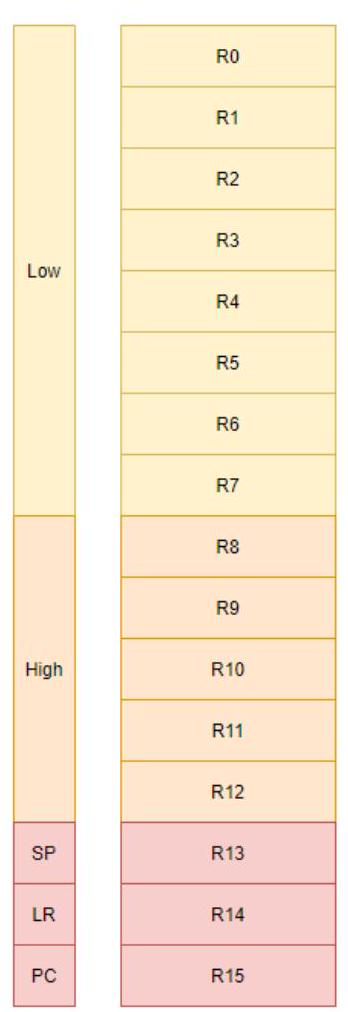
\includegraphics[width=0.35\linewidth, angle=90]{images/2024_12_29_79e6b22f503fb7b4f718g-02}

Main instruction types:
\begin{itemize}
  \item \textbf{Data Transfer}: Move, Load, Store operations
  \item \textbf{Data Processing}: Arithmetic, logical, shift operations
  \item \textbf{Control Flow}: Branch and function calls
\end{itemize}
\end{definition}

\begin{code}{Basic Assembly Program Structure}
Example of a simple assembly program:
\begin{lstlisting}[language=armasm, style=basesmol]
Label   Instr.  Operands   Comments
demoprg MOVS    R0,#0xA5   ;copy 0xA5 into R0
        MOVS    R1,#0x11   ;copy 0x11 into R1
        ADDS    R0,R0,R1   ;add R0 and R1, store in R0
\end{lstlisting}
\end{code}

\begin{concept}{Assembly Program Sections}\\
Program memory is organized in sections:

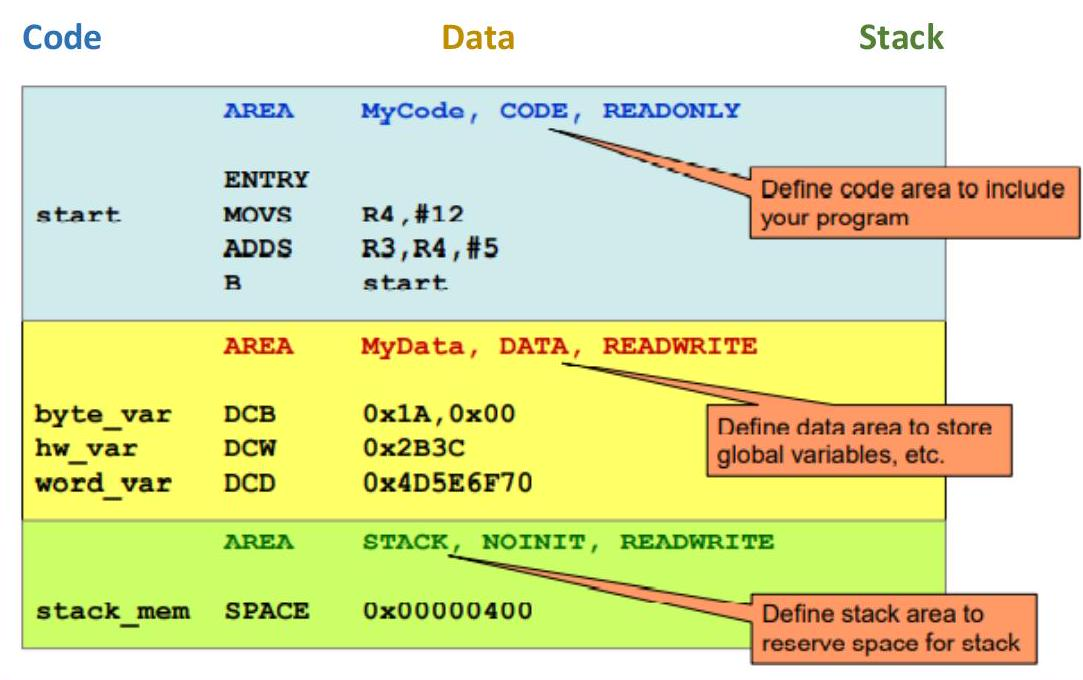
\includegraphics[width=\linewidth]{images/2024_12_29_79e6b22f503fb7b4f718g-02(1)}

\textbf{Directives for initialized data:}
\begin{itemize}
  \item \textbf{DCB}: Define Constant Byte (8-bit)
  \item \textbf{DCW}: Define Constant Half-Word (16-bit)
  \item \textbf{DCD}: Define Constant Word (32-bit)
\end{itemize}

\textbf{Directive for uninitialized data:}
\begin{itemize}
  \item \textbf{SPACE}: Reserve specified number of bytes
\end{itemize}
\end{concept}

\begin{code}{Data Definition}
Memory layout for different data types:
\begin{lstlisting}[language=armasm, style=basesmol]
var1    DCB     0x1A                ;single byte
var2    DCB     0x2B,0x3C,0x4D,0x5E ;byte array
var3    DCW     0x6F70,0x8192       ;half-words
var4    DCD     0xA3B4C5D6          ;word
data    SPACE   100                 ;reserve 100 bytes
\end{lstlisting}
\end{code}

\begin{KR}{Creating Assembly Programs}\\
Steps to create an assembly program:
\begin{enumerate}
  \item Define program sections (CODE, DATA)
  \item Declare any external symbols (IMPORT/EXPORT)
  \item Define initialized data using DCx directives
  \item Reserve uninitialized data using SPACE
  \item Write program code using proper instruction syntax
  \item End program with END directive
\end{enumerate}
\end{KR}
	\raggedcolumns
	\section{Data Transfer}

\begin{concept}{Data Transfer Overview}\\
ARM Cortex-M uses a load/store architecture:
\begin{itemize}
  \item Memory can only be accessed through load and store instructions
  \item All other operations work on registers
  \item Various addressing modes for flexible memory access
\end{itemize}
\end{concept}

\begin{formula}{Load Instructions}\\
Main load instructions for moving data into registers:
\begin{itemize}
  \item \textbf{MOVS} (Move and Set flags):
    \begin{itemize}
      \item Register to Register: \texttt{MOVS R1, R2}
      \item 8-bit immediate: \texttt{MOVS R1, \#0x1C}
      \item Constant: \texttt{MOVS R1, \#MyConst}
    \end{itemize}
  \item \textbf{LDR} (Load Register):
    \begin{itemize}
      \item 32-bit literal: \texttt{LDR R1, \#0xA1B2C3D4}
      \item PC-relative: \texttt{LDR R1, [PC, \#12]}
      \item Pseudo instruction: \texttt{LDR R1, =MyConst}
      \item Register indirect: \texttt{LDR R1, [R2]}
    \end{itemize}
  \item \textbf{LDRB} (Load Register Byte):
    \begin{itemize}
      \item Loads 8-bit value
      \item Bits 31 to 8 are set to zero
    \end{itemize}
  \item \textbf{LDRH} (Load Register Half-word):
    \begin{itemize}
      \item Loads 16-bit value
      \item Bits 31 to 16 are set to zero
    \end{itemize}
\end{itemize}
\end{formula}

\begin{formula}{Store Instructions}\\
Instructions for storing data from registers to memory:
\begin{itemize}
  \item \textbf{STR} (Store Register):
    \begin{itemize}
      \item Basic store: \texttt{STR R1, [R2]}
      \item With offset: \texttt{STR R1, [R2, \#0x04]}
    \end{itemize}
  \item \textbf{STRB} (Store Register Byte):
    \begin{itemize}
      \item Stores lowest 8 bits of register
    \end{itemize}
  \item \textbf{STRH} (Store Register Half-word):
    \begin{itemize}
      \item Stores lowest 16 bits of register
    \end{itemize}
\end{itemize}
\end{formula}

\begin{example2}{Memory Access Example}\\
Loading and storing array elements:

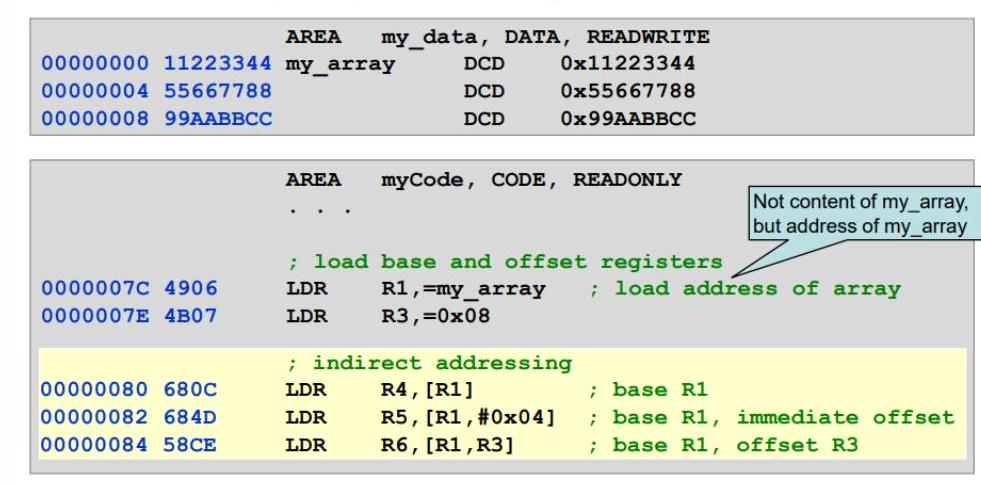
\includegraphics[width=\linewidth]{images/2024_12_29_79e6b22f503fb7b4f718g-03(1)}
\end{example2}

\begin{example2}{Memory Layout Example}\\
Memory layout for array elements and instructions:

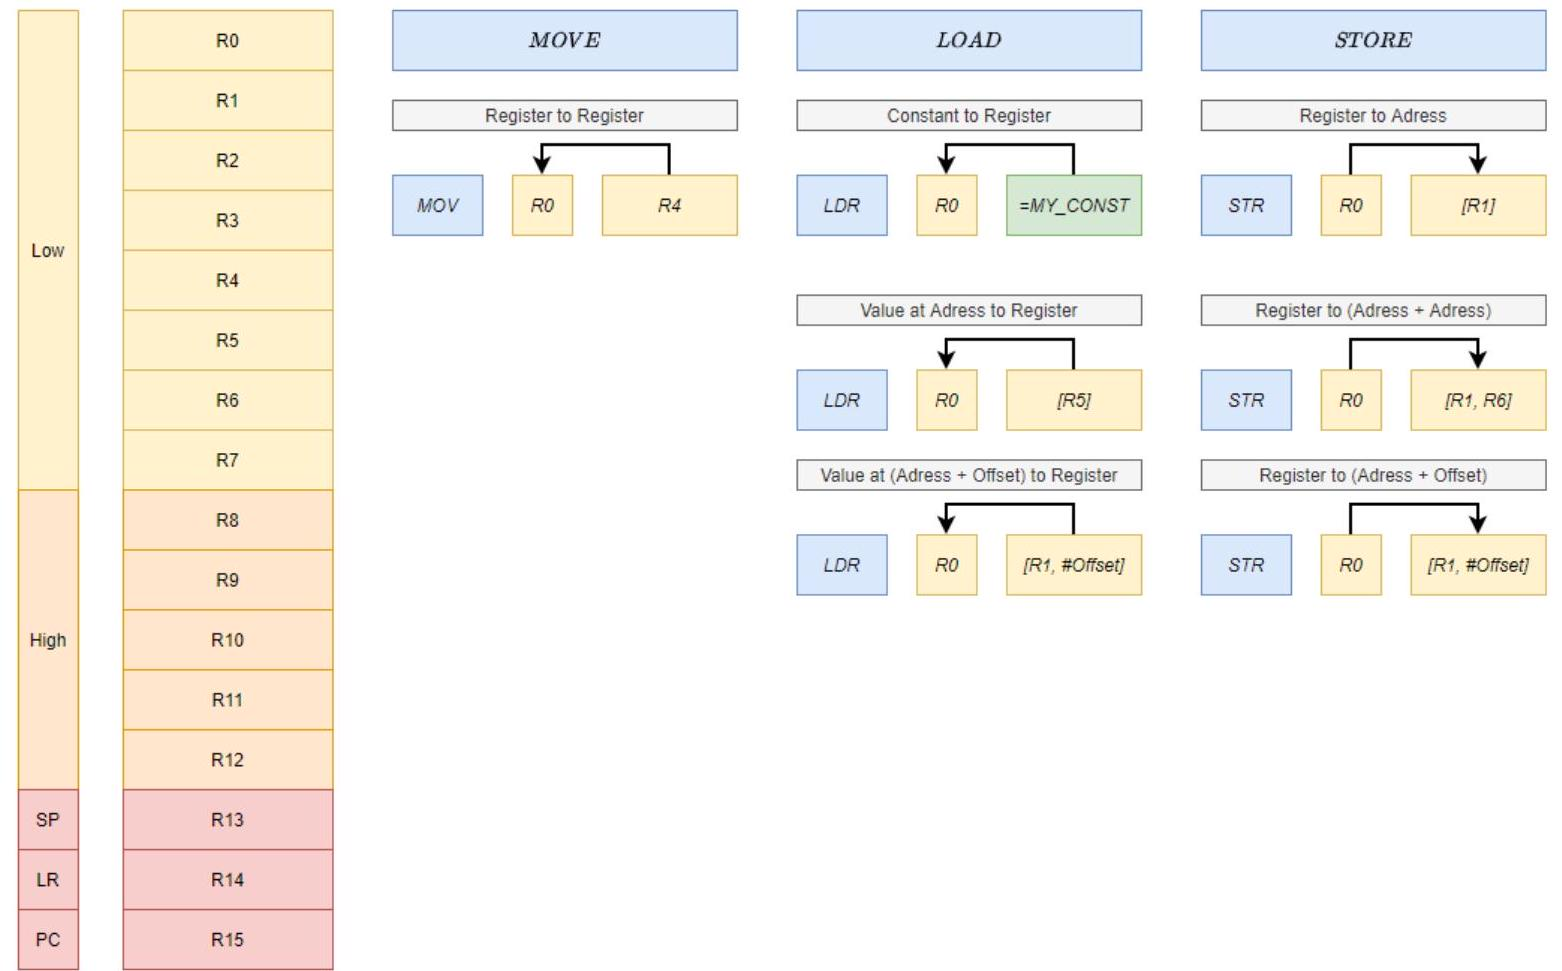
\includegraphics[width=\linewidth]{images/2024_12_29_79e6b22f503fb7b4f718g-03}
\end{example2}
\begin{remark}
Size considerations:
\begin{itemize}
  \item Array elements: 3 * 4 Bytes
  \item Instructions: 5 * 2 Bytes
  \item Literals (0x08): 1 * 4 Bytes
\end{itemize}
\end{remark}

\begin{KR}{Memory Access Patterns}\\
Steps for accessing memory:
\begin{enumerate}
  \item Determine required data size (byte, half-word, word)
  \item Choose appropriate load/store instruction
  \item Calculate correct memory address
  \item Consider alignment requirements
  \item Load/store data using proper addressing mode
\end{enumerate}
\end{KR}

\begin{example2}{Basic Data Transfer Operations}
Common data transfer operations:
\begin{lstlisting}[language=armasm, style=basesmol]
;Load operations
MOVS R1, #42      ;Load immediate value
MOVS R2, R1       ;Copy register
LDR  R3, =0x1234  ;Load 32-bit constant
LDR  R4, [R3]     ;Load from memory
LDRB R5, [R3, #1] ;Load byte with offset

;Store operations
STR  R1, [R2]     ;Store word
STRB R1, [R2, #4] ;Store byte with offset
STRH R1, [R2, R3] ;Store half-word with register offset
\end{lstlisting}
\end{example2}
	\raggedcolumns
	\section{Arithmetic Operations}

\begin{concept}{Processor Status Flags}\\
APSR (Application Program Status Register) contains important flags affected by arithmetic operations:
\begin{itemize}
  \item \textbf{N} (Negative): Set when result's MSB = 1, used for signed operations
  \item \textbf{Z} (Zero): Set when result = 0, used for both signed/unsigned
  \item \textbf{C} (Carry): Set when unsigned overflow occurs
  \item \textbf{V} (Overflow): Set when signed overflow occurs
\end{itemize}

Instructions ending with 'S' modify these flags:
\begin{itemize}
  \item ADDS, SUBS, MOVS, LSLS
\end{itemize}
\end{concept}

\begin{definition}{Basic Arithmetic Instructions}\\
Core arithmetic operations:
\begin{itemize}
  \item \textbf{ADD/ADDS}: Addition ($A + B$)
  \item \textbf{ADCS}: Addition with Carry ($A + B + c$)
  \item \textbf{ADR}: Address to Register ($PC + A$)
  \item \textbf{SUB/SUBS}: Subtraction ($A - B$)
  \item \textbf{SBCS}: Subtraction with carry/borrow ($A - B - !c$)
  \item \textbf{RSBS}: Reverse Subtract ($-1 \cdot A$)
  \item \textbf{MULS}: Multiplication ($A \cdot B$)
\end{itemize}
\end{definition}

\begin{definition}{Two's Complement}\\
For negative numbers:
\begin{itemize}
  \item Two's complement: $A = !A + 1$
  \item Used for representing signed numbers
  \item Enables using same hardware for addition and subtraction
\end{itemize}
\end{definition}

\begin{concept}{Carry and Overflow}\\
\textbf{Unsigned Operations:}
\begin{itemize}
  \item Addition: C = 1 indicates carry (result too large)
  \item Subtraction: C = 0 indicates borrow (result negative)
\end{itemize}

\textbf{Signed Operations:}
\begin{itemize}
  \item Addition: V = 1 if overflow with operands of same sign
  \item Subtraction: V = 1 if overflow with operands of opposite signs
\end{itemize}
\end{concept}

\begin{example2}{Multi-Word Addition}
Adding 96-bit values using ADCS:

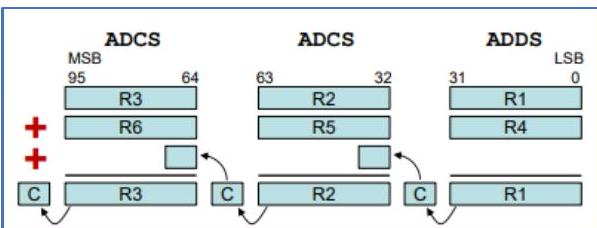
\includegraphics[width=\linewidth]{images/2024_12_29_79e6b22f503fb7b4f718g-04}

\begin{lstlisting}[language=armasm, style=basesmol]
    ADDS R1, R1, R4    ; Add least significant words
    ADCS R2, R2, R5    ; Add middle words with carry
    ADCS R3, R3, R6    ; Add most significant words with carry
\end{lstlisting}
\end{example2}

\begin{example2}{Multi-Word Subtraction}
Subtracting 96-bit values using SBCS:

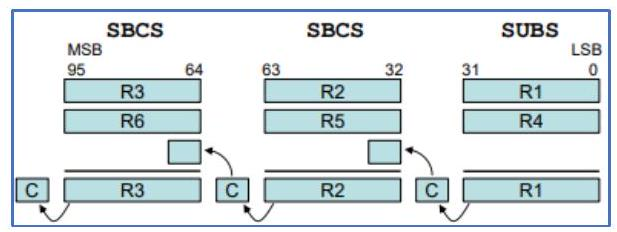
\includegraphics[width=\linewidth]{images/2024_12_29_79e6b22f503fb7b4f718g-04(1)}

\begin{lstlisting}[language=armasm, style=basesmol]
    SUBS R1, R1, R4    ; Subtract least significant words
    SBCS R2, R2, R5    ; Subtract middle words with borrow
    SBCS R3, R3, R6    ; Subtract most significant words with borrow
\end{lstlisting}
\end{example2}

\begin{example2}{Addition and Subtraction Examples}
Addition with carry (13d + 7d):
\begin{verbatim}
  1101  (13d)
  0111  (7d)
  ----
1 0100  (20d = 16d + 4d)
\end{verbatim}

Subtraction with borrow (6d - 14d):
\begin{verbatim}
  0110  (6d)
+ 0010  (TC of 14d)
  ----
  1000  (8d - 16d = -8d)
\end{verbatim}

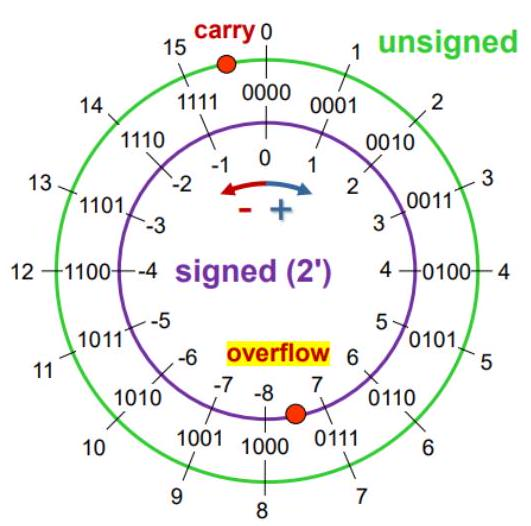
\includegraphics[width=\linewidth]{images/2024_12_29_79e6b22f503fb7b4f718g-04(2)}
\end{example2}

\begin{KR}{Arithmetic Operations}\\
Steps for arithmetic operations:
\begin{enumerate}
  \item Determine if operation is signed or unsigned
  \item Choose appropriate instruction (with or without 'S')
  \item Consider potential carry/overflow conditions
  \item For multi-word operations:
    \begin{itemize}
      \item Start with least significant words
      \item Use carry-aware instructions for higher words
      \item Track flags through operation
    \end{itemize}
  \item Check relevant flags after operation
\end{enumerate}
\end{KR}
	\section{Logic, Shift and Rotate Instructions}

\begin{concept}{Logic Instructions}\\
Base logic operations (affect only N and Z flags):
\begin{itemize}
  \item \textbf{ANDS}: Bitwise AND (Rdn \& Rm, a \& b)
  \item \textbf{BICS}: Bit Clear (Rdn \& !Rm, a \& ~b)
  \item \textbf{EORS}: Exclusive OR (Rdn \textdollar Rm, a $\wedge$  b)
  \item \textbf{MVNS}: Bitwise NOT (!Rm, ~a)
  \item \textbf{ORRS}: Bitwise OR (Rdn \# Rm, a | b)
\end{itemize}
\end{concept}

\begin{example2}{Logical Operations}
Common logic operations:
\begin{lstlisting}[language=armasm, style=basesmol]
; Logic operations
ANDS R0, R1         ; R0 = R0 AND R1
BICS R0, R1         ; R0 = R0 AND NOT R1
EORS R0, R1         ; R0 = R0 XOR R1
MVNS R0, R1         ; R0 = NOT R1
ORRS R0, R1         ; R0 = R0 OR R1

; Shift operations
LSLS R0, R1, #2     ; R0 = R1 << 2 (multiply by 4)
LSRS R0, R1, #1     ; R0 = R1 >> 1 (divide by 2)
ASRS R0, R1, #2     ; R0 = R1 >> 2 (signed divide by 4)
RORS R0, R1, #1     ; Rotate R1 right by 1 bit
\end{lstlisting}
\end{example2}

\begin{concept}{Shift and Rotate Instructions}\\
Shift operations for binary manipulation:
\begin{itemize}
  \item \textbf{LSLS}: Logical Shift Left ($2^n \cdot Rn$, 0 $\rightarrow$ LSB)
  \item \textbf{LSRS}: Logical Shift Right ($2^{-n} \cdot Rn$, 0 $\rightarrow$ MSB)
  \item \textbf{ASRS}: Arithmetic Shift Right ($R^{-n}$, ±MSB $\rightarrow$ MSB)
  \item \textbf{RORS}: Rotate Right (LSB $\rightarrow$ MSB)
\end{itemize}

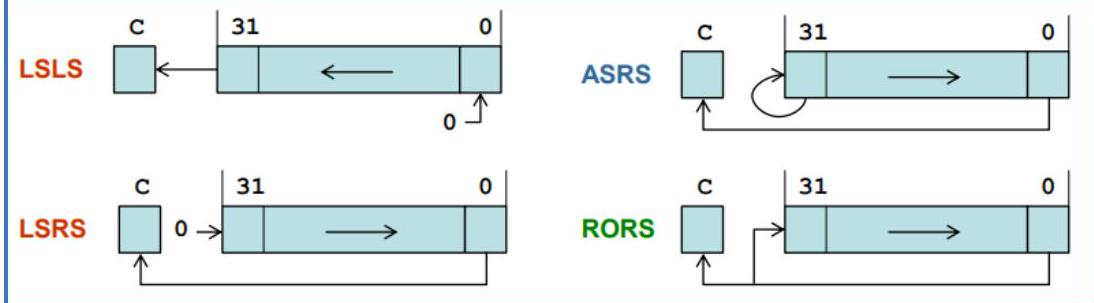
\includegraphics[width=\linewidth]{images/2024_12_29_79e6b22f503fb7b4f718g-06}
\end{concept}

\begin{example2}{Shift Operations for Arithmetic}
Using shifts for multiplication and division:
\begin{lstlisting}[language=armasm, style=basesmol]
; Multiplication by powers of 2
LSLS    R0, R0, #1      ; R0 = R0 * 2
LSLS    R0, R0, #2      ; R0 = R0 * 4
LSLS    R0, R0, #3      ; R0 = R0 * 8

; Division by powers of 2
LSRS    R0, R0, #1      ; R0 = R0 / 2 (unsigned)
ASRS    R0, R0, #1      ; R0 = R0 / 2 (signed)

; Multiply by 10 (8 + 2)
LSLS    R1, R0, #3      ; R1 = R0 * 8
ADDS    R0, R0, R1      ; R0 = R0 + (R0 * 8) = R0 * 9
ADDS    R0, R0, R0      ; R0 = R0 * 2 = R0 * 10
\end{lstlisting}
\end{example2}



\begin{KR}{Using Logic and Shift Instructions}
Steps for bit manipulation:
\begin{enumerate}
  \item Identify required operation (AND, OR, XOR, NOT, shift)
  \item Choose appropriate instruction
  \item Consider effect on flags if relevant
\end{enumerate}

\begin{minipage}[t]{0.55\textwidth}
  \textbf{For shifts:}
    \begin{itemize}
      \item LSLS for multiplication by $2^n$
      \item LSRS for unsigned division by $2^n$
      \item ASRS for signed division by $2^n$
    \end{itemize}
\end{minipage}
\begin{minipage}[t]{0.4\textwidth}
  \textbf{For logic:}
    \begin{itemize}
      \item ANDS for bit masking
      \item ORRS for bit setting
      \item BICS for bit clearing
      \item EORS for bit toggling
    \end{itemize}
\end{minipage}
\end{KR}

\begin{concept}{Flag Behavior with Logic Instructions}\\
Logic instructions only affect N and Z flags:
\begin{itemize}
  \item \textbf{N flag}: Set to bit 31 of result (MSB)
  \item \textbf{Z flag}: Set if result is zero
  \item \textbf{C, V flags}: Unchanged
\end{itemize}

Special case for shift/rotate:
\begin{itemize}
  \item \textbf{C flag}: Set to last bit shifted out
  \item \textbf{N,Z flags}: Set based on result
  \item \textbf{V flag}: Unchanged
\end{itemize}
\end{concept}

\begin{KR}{Bit Manipulation Techniques}\\
Common patterns for bit manipulation:

1. Setting specific bits:
\begin{lstlisting}[language=armasm, style=basesmol]
MOVS    R0, #pattern    ; Create bit pattern
ORRS    target, R0      ; OR to set bits
\end{lstlisting}

2. Clearing specific bits:
\begin{lstlisting}[language=armasm, style=basesmol]
MOVS    R0, #pattern    ; Create bit pattern
BICS    target, R0      ; Clear selected bits
\end{lstlisting}

3. Inverting specific bits:
\begin{lstlisting}[language=armasm, style=basesmol]
MOVS    R0, #pattern    ; Create bit pattern
EORS    target, R0      ; XOR to invert bits
\end{lstlisting}

4. Testing bits:
\begin{lstlisting}[language=armasm, style=basesmol]
MOVS    R0, #pattern    ; Create bit pattern
ANDS    R1, target, R0  ; AND to test bits
; Check flags for result
\end{lstlisting}
\end{KR}

\begin{example2}{Bit Manipulation}
\begin{lstlisting}[language=armasm, style=basesmol]
; Set bits 0 and 4
MOVS    R1, #0x11       ; Mask: 0001 0001
ORRS    R0, R1          ; Set bits in R0

; Clear bits 1 and 5
MOVS    R1, #0x22       ; Mask: 0010 0010
BICS    R0, R1          ; Clear bits in R0

; Toggle bits 2,3,4
MOVS    R1, #0x1C       ; Mask: 0001 1100
EORS    R0, R1          ; Toggle bits in R0

; Test bit 3
MOVS    R1, #0x08       ; Mask: 0000 1000
ANDS    R2, R0, R1      ; Test bit
BEQ     bit_is_clear    ; Branch if bit was 0
\end{lstlisting}
\end{example2}





\subsubsection{Casting, Sign Extension and Type Conversion}

\begin{definition}{Integer Casting}\\
\textbf{Extension (adding bits):}

\begin{minipage}{0.5\textwidth}
\begin{itemize}
  \item \textbf{Zero Extension} (unsigned):
    \begin{itemize}
      \item Fill left bits with zero
      \item Example: 1011 $\rightarrow$ 00001011
    \end{itemize}
\end{itemize}
\end{minipage}
\begin{minipage}{0.5\textwidth}
\begin{itemize}
  \item \textbf{Sign Extension} (signed):
    \begin{itemize}
      \item Copy sign bit to the left
      \item Example: 1011 $\rightarrow$ 11111011
    \end{itemize}
\end{itemize}
\end{minipage}

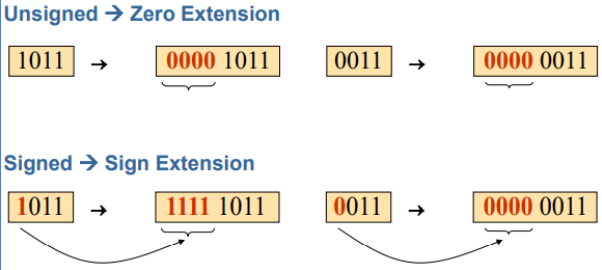
\includegraphics[width=0.7\linewidth]{images/sign_extension.png}

\textbf{Truncation:} Cast cuts out the left most bits
\begin{itemize}
  \item Signed: May change sign
  \item Unsigned: Results in modulo operation
\end{itemize}
\end{definition}

\begin{formula}{Integer Ranges based on word size}\\
  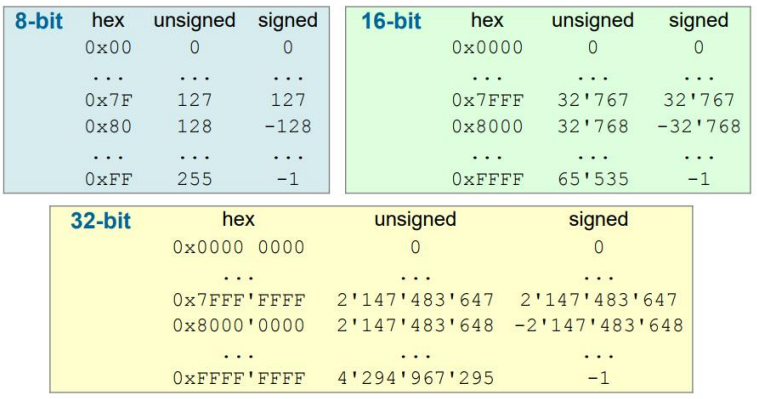
\includegraphics[width=\linewidth]{images/integer_ranges.png}
\end{formula}



\begin{concept}{Sign Extension Instructions}\\
Instructions for extending smaller values:

\begin{minipage}{0.5\textwidth}
\textbf{SXTB}: Sign extend byte to word
    \begin{itemize}
      \item Takes lowest byte
      \item Copies bit 7 to bits 31-8
    \end{itemize}
\textbf{SXTH}: \\Sign extend half-word to word
    \begin{itemize}
      \item Takes lowest half-word
      \item Copies bit 15 to bits 31-16
    \end{itemize}
\end{minipage}
\begin{minipage}{0.5\textwidth}
\textbf{UXTB}: Zero extend byte to word
    \begin{itemize}
      \item Takes lowest byte
      \item Sets bits 31-8 to zero
    \end{itemize}
\textbf{UXTH}:\\ Zero extend half-word to word
    \begin{itemize}
      \item Takes lowest half-word
      \item Sets bits 31-16 to zero
    \end{itemize}
\end{minipage}
\end{concept}

\begin{example2}{Sign Examples}
\begin{lstlisting}[language=armasm, style=basesmol]
; Sign extension examples
SXTB    R0, R1          ; Sign extend byte
SXTH    R0, R1          ; Sign extend half-word

; Zero extension examples
UXTB    R0, R1          ; Zero extend byte
UXTH    R0, R1          ; Zero extend half-word

; Manual sign extension
LSLS    R0, R0, #24     ; Shift left 24 bits
ASRS    R0, R0, #24     ; Arithmetic shift right 24
\end{lstlisting}
\end{example2}

\begin{KR}{Type Conversion Guidelines}
Steps for safe type conversion:

1. For unsigned to larger unsigned:
\begin{itemize}
  \item Use zero extension (UXTB, UXTH)
  \item Or use LSLS followed by LSRS
\end{itemize}

\begin{lstlisting}[language=armasm, style=basesmol]
  ; Extend 8-bit to 32-bit unsigned
  MOVS    R0, #0xFF       ; Load 8-bit value
  UXTB    R2, R0          ; Unsigned extension
  
  ; Manual zero extension
  LDRB    R0, [R1]       ; Load byte, top bits zero
  LSLS    R0, #24        ; Move to top byte
  LSRS    R0, #24        ; Logical shift back
\end{lstlisting}

2. For signed to larger signed:
\begin{itemize}
  \item Use sign extension (SXTB, SXTH)
  \item Or use LSLS followed by ASRS
\end{itemize}

\begin{lstlisting}[language=armasm, style=basesmol]
  ; Extend 8-bit to 32-bit signed
  MOVS    R0, #0xFF       ; Load 8-bit value
  SXTB    R1, R0          ; Signed extension
  
  ; Manual sign extension
  LDRSB   R0, [R1]       ; Load with sign extend
  LDRB    R0, [R1]       ; Load byte
  LSLS    R0, #24        ; Move to top byte
  ASRS    R0, #24        ; Arithmetic shift back
\end{lstlisting}


3. Reducing size (truncation):
\begin{itemize}
  \item Use AND with appropriate mask
  \item Or store using STRB/STRH
  \item Check for potential data loss
\end{itemize}


Example:
\begin{lstlisting}[language=armasm, style=basesmol]
    ; Truncate 32-bit to 8-bit
    MOVS    R1, #0xFF       ; Create mask
    ANDS    R0, R1          ; Truncate to 8 bits

    ; Store 32-bit value as 8-bit
    STRB    R0, [R1]        ; Store byte 
\end{lstlisting}
%TODO: check if this is correct
\end{KR}


\raggedcolumns

\begin{remark}
Important considerations:
\begin{itemize}
  \item Always consider signedness of values
  \item Check for potential carry/overflow in arithmetic shifts
  \item Remember carry flag behavior in shifts
  \item Use appropriate extension for data type
  \item Consider performance impact of shifts vs multiply
  \item Be careful with bit patterns crossing byte boundaries
  \item Document complex bit manipulations clearly
\end{itemize}
\end{remark}




	\section{Control Structures}

\begin{concept}{Branch Instructions}\\
Branch instructions control program flow:

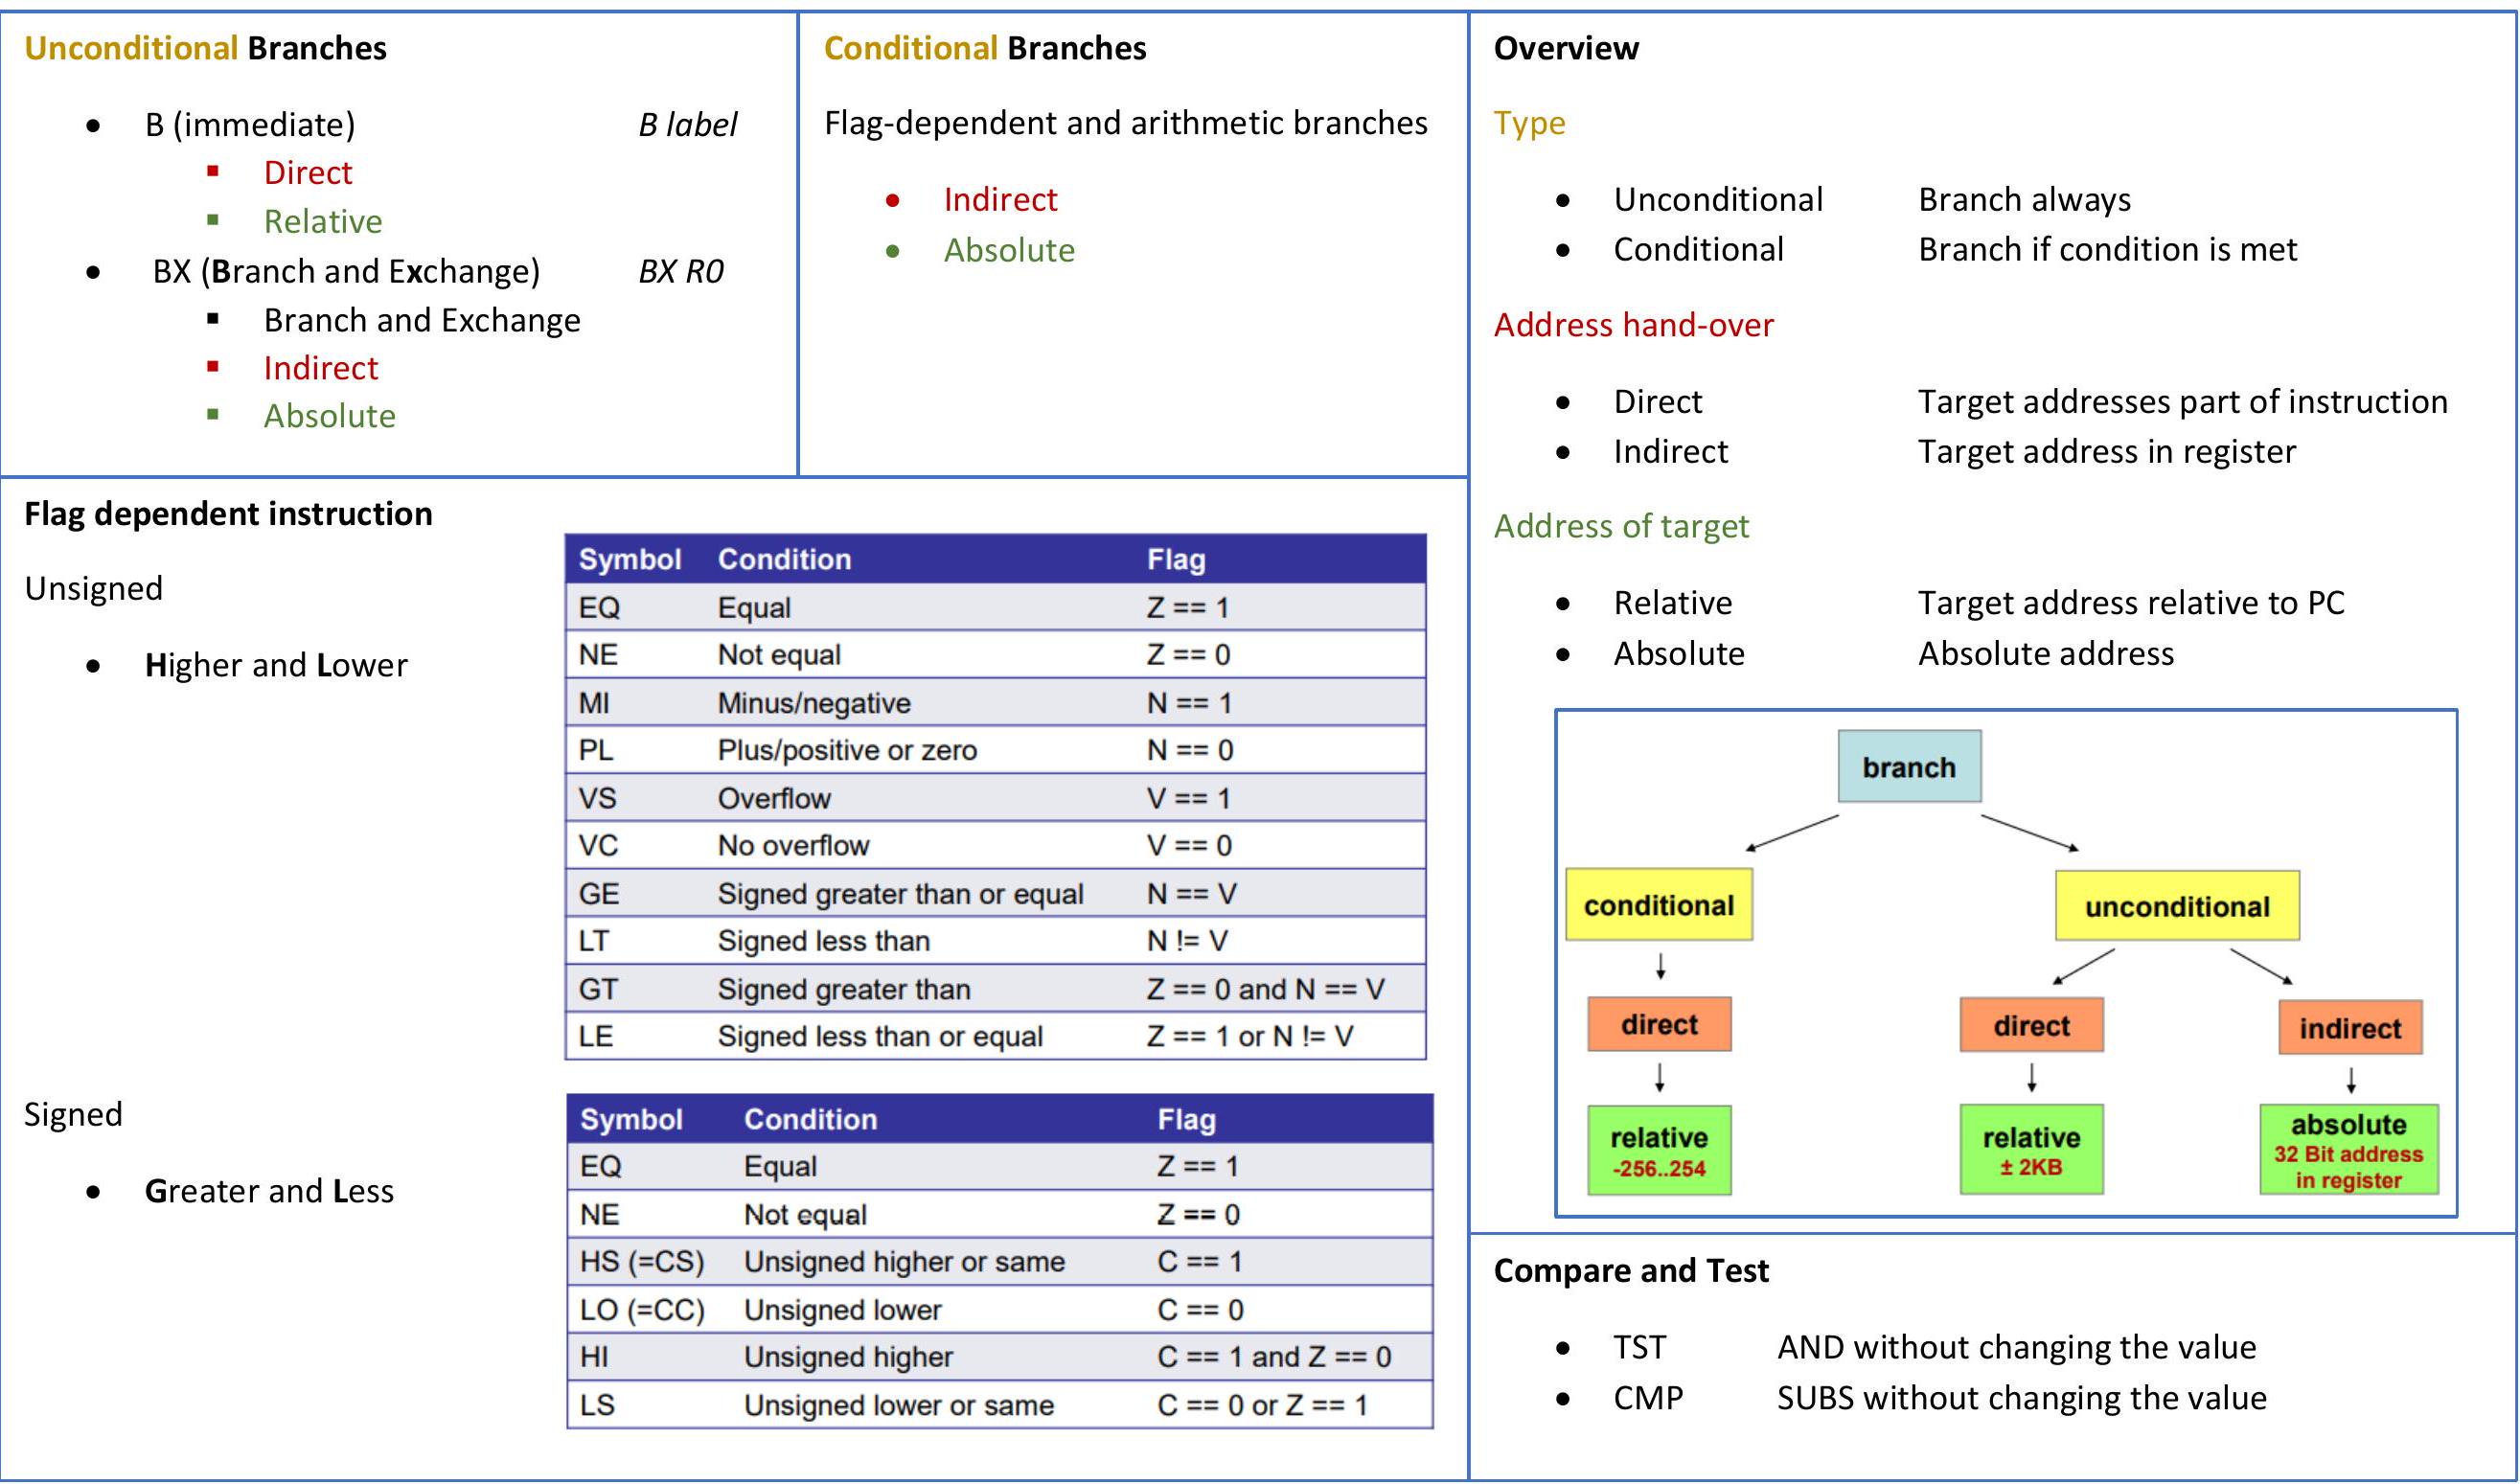
\includegraphics[width=\linewidth]{images/2024_12_29_79e6b22f503fb7b4f718g-05}

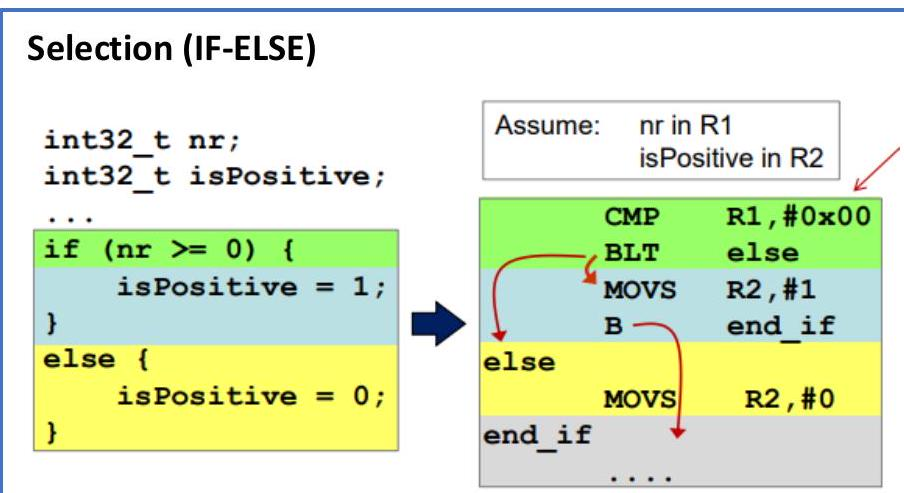
\includegraphics[width=\linewidth]{images/2024_12_29_79e6b22f503fb7b4f718g-07(3)}
\end{concept}

\begin{example2}{Switch Statement Implementation}
C code example:
\begin{lstlisting}[language=C, style=basesmol]
uint32_t result, n;
switch (n) {
    case 0:
        result += 17;
        break;
    case 1:
        result += 13;
        //fall through
    case 3: 
    case 5:
        result += 37;
        break;
    default:
        result = 0;
}
\end{lstlisting}

Assembly implementation with jump table:
\begin{lstlisting}[language=armasm, style=basesmol]
NR_CASES    EQU     6
case_switch CMP     R1, #NR_CASES
            BHS     case_default
            LSLS    R1, #2        ; * 4
            LDR     R7, =jump_table
            LDR     R7, [R7, R1]
            BX      R7

case_0      ADDS    R2, R2, #17
            B       end_sw_case
case_1      ADDS    R2, R2, #13
case_3_5    ADDS    R2, R2, #37
            B       end_sw_case
case_default MOVS   R2, #0
end_sw_case ...

jump_table  DCD     case_0
            DCD     case_1
            DCD     case_default
            DCD     case_3_5
            DCD     case_default
            DCD     case_3_5
\end{lstlisting}
\end{example2}

\begin{concept}{Loop Types}\\
Three main types of loops:

\textbf{Do-While (Post-Test Loop)}:
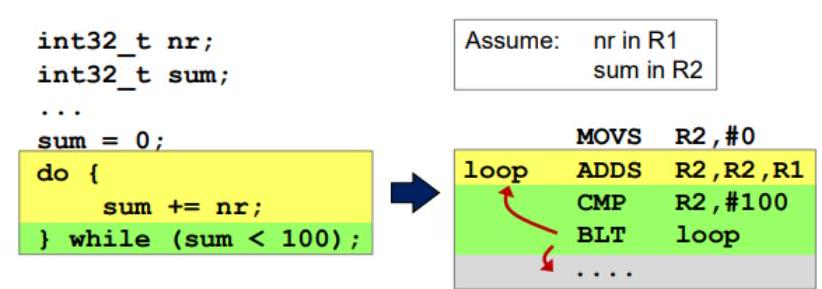
\includegraphics[width=\linewidth]{images/2024_12_29_79e6b22f503fb7b4f718g-07}

\textbf{While (Pre-Test Loop)}:
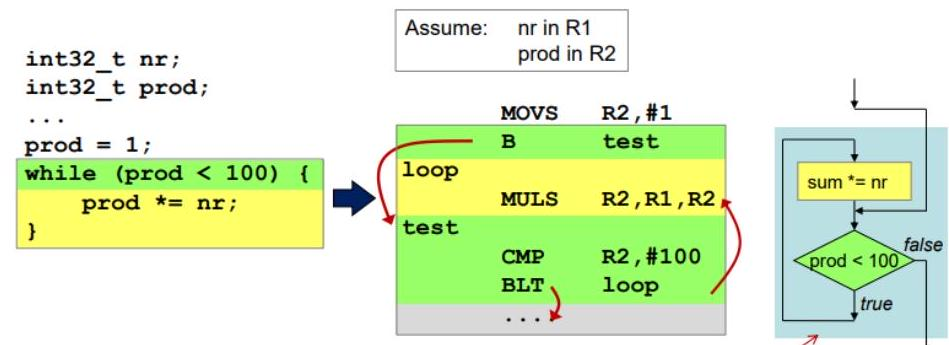
\includegraphics[width=\linewidth]{images/2024_12_29_79e6b22f503fb7b4f718g-07(1)}

\textbf{For Loop (Pre-Test Loop)}:
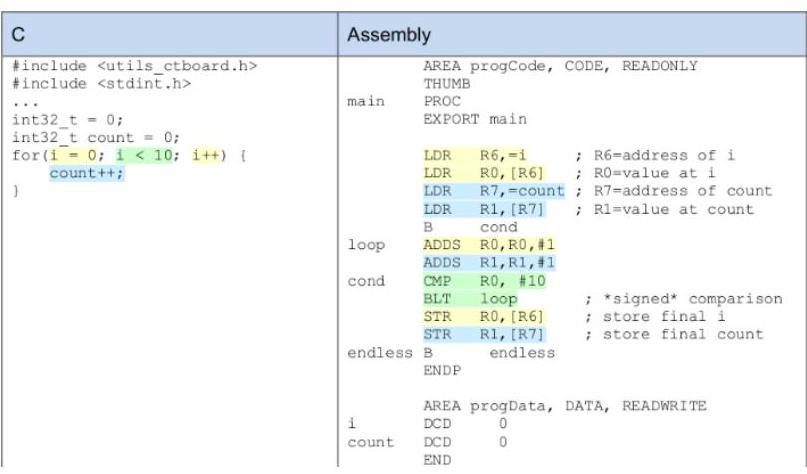
\includegraphics[width=\linewidth]{images/2024_12_29_79e6b22f503fb7b4f718g-07(2)}
\end{concept}

\begin{KR}{Implementing Control Structures}\\
Steps for implementing control structures:
\begin{enumerate}
  \item Choose appropriate control structure:
    \begin{itemize}
      \item If-then-else for simple decisions
      \item Switch for multiple cases with same variable
      \item Loops for repeated operations
    \end{itemize}
  \item For switches:
    \begin{itemize}
      \item Create jump table
      \item Calculate offset based on case value
      \item Handle default case
    \end{itemize}
  \item For loops:
    \begin{itemize}
      \item Initialize counter/condition
      \item Place condition check appropriately
      \item Ensure proper exit condition
      \item Update variables correctly
    \end{itemize}
\end{enumerate}
\end{KR}

\begin{example2}{Basic Control Structures}
Example implementations:
\begin{lstlisting}[language=armasm, style=basesmol]
    ; If-then-else
    CMP     R0, #0      ; Compare value
    BEQ     else_label  ; Branch if equal
    ; then code
    B       endif_label
else_label
    ; else code
endif_label

    ; While loop
    B       while_cond  ; Jump to condition
while_loop
    ; loop body
while_cond
    CMP     R0, #10     ; Check condition
    BLT     while_loop  ; Branch if less than

    ; Do-while loop
do_loop
    ; loop body
    CMP     R0, #10     ; Check condition
    BLT     do_loop     ; Branch if less than
\end{lstlisting}
\end{example2}

\begin{formula}{Branch Instruction Types}\\
Classification of branch instructions:

\textbf{1. Based on Condition:}
\begin{itemize}
  \item \textbf{Unconditional:}
    \begin{itemize}
      \item B - Branch always
      \item BL - Branch with Link
      \item BX - Branch and Exchange
    \end{itemize}
  \item \textbf{Conditional:}
    \begin{itemize}
      \item Flag-dependent (EQ, NE, CS, CC, etc.)
      \item Arithmetic (HI, LS, GE, LT, etc.)
    \end{itemize}
\end{itemize}

\textbf{2. Based on Target Address:}
\begin{itemize}
  \item \textbf{Direct:} Target address in instruction
  \item \textbf{Indirect:} Target address in register
  \item \textbf{Relative:} Offset from current PC
  \item \textbf{Absolute:} Complete target address
\end{itemize}
\end{formula}

\begin{KR}{Selection Implementation}\\
Guidelines for implementing if-then-else structures:

1. Simple if-then:
\begin{lstlisting}[language=armasm, style=basesmol]
    ; if (x > 0) { x++; }
    CMP     R0, #0          ; Compare x with 0
    BLE     endif           ; Skip if x <= 0
    ADDS    R0, #1          ; x++
endif
\end{lstlisting}

2. if-then-else:
\begin{lstlisting}[language=armasm, style=basesmol]
    ; if (x > y) { x = y; } else { y = x; }
    CMP     R0, R1          ; Compare x and y
    BLE     else_part       ; Branch if x <= y
    MOVS    R0, R1          ; Then part: x = y
    B       endif           ; Skip else part
else_part
    MOVS    R1, R0          ; Else part: y = x
endif
\end{lstlisting}

3. Nested if:
\begin{lstlisting}[language=armasm, style=basesmol]
    ; if (x > 0) {
    ;     if (y > 0) {
    ;         x = y;
    ;     }
    ; }
    CMP     R0, #0          ; Check x > 0
    BLE     endif_outer
    CMP     R1, #0          ; Check y > 0
    BLE     endif_inner
    MOVS    R0, R1          ; x = y
endif_inner
endif_outer
\end{lstlisting}
\end{KR}

\begin{KR}{Loop Implementation}\\
Templates for different loop types:

1. While loop:
\begin{lstlisting}[language=armasm, style=basesmol]
    ; while (x < 10) { x++; }
    B       while_cond      ; Jump to condition
while_loop
    ADDS    R0, #1          ; x++
while_cond
    CMP     R0, #10         ; Check x < 10
    BLT     while_loop      ; Continue if true
\end{lstlisting}

2. Do-while loop:
\begin{lstlisting}[language=armasm, style=basesmol]
    ; do { x++; } while (x < 10);
do_loop
    ADDS    R0, #1          ; x++
    CMP     R0, #10         ; Check x < 10
    BLT     do_loop         ; Continue if true
\end{lstlisting}

3. For loop:
\begin{lstlisting}[language=armasm, style=basesmol]
    ; for (i = 0; i < 10; i++)
    MOVS    R0, #0          ; i = 0
    B       for_cond
for_loop
    ; Loop body
    ADDS    R0, #1          ; i++
for_cond
    CMP     R0, #10         ; Check i < 10
    BLT     for_loop        ; Continue if true
\end{lstlisting}
\end{KR}

\begin{KR}{Switch Implementation}\\
Steps for implementing switch statements:

1. Range check and table access:
\begin{lstlisting}[language=armasm, style=basesmol]
    CMP     R0, #MAX_CASES  ; Check range
    BHS     default_case    ; If too high, default
    LSLS    R0, #2          ; Multiply by 4
    LDR     R1, =jump_table ; Load table address
    ADD     R1, R0          ; Add offset
    LDR     R1, [R1]        ; Load target address
    BX      R1              ; Branch to case
\end{lstlisting}

2. Jump table structure:
\begin{lstlisting}[language=armasm, style=basesmol]
jump_table
    DCD     case_0          ; Case 0 handler
    DCD     case_1          ; Case 1 handler
    DCD     default_case    ; Default handler
    ; ... more cases
\end{lstlisting}

3. Case handlers:
\begin{lstlisting}[language=armasm, style=basesmol]
case_0
    ; Handle case 0
    B       switch_end
case_1
    ; Handle case 1
    B       switch_end
default_case
    ; Handle default case
switch_end
\end{lstlisting}
\end{KR}

\begin{example2}{Complex Control Structure}
Implementing nested loops with conditions:
\begin{lstlisting}[language=armasm, style=basesmol]
    ; for (i = 0; i < 5; i++) {
    ;     if (i == 2) continue;
    ;     for (j = 0; j < 3; j++) {
    ;         if (j == 1) break;
    ;         sum += i + j;
    ;     }
    ; }
    
    MOVS    R0, #0          ; i = 0
outer_loop
    CMP     R0, #2          ; Check i == 2
    BEQ     outer_continue  ; Skip if i == 2
    
    MOVS    R1, #0          ; j = 0
inner_loop
    CMP     R1, #1          ; Check j == 1
    BEQ     outer_continue  ; Break to outer loop
    
    ADDS    R2, R0, R1      ; Calculate i + j
    ADDS    R4, R4, R2      ; Add to sum
    
    ADDS    R1, #1          ; j++
    CMP     R1, #3          ; Check j < 3
    BLT     inner_loop      ; Continue inner loop
    
outer_continue
    ADDS    R0, #1          ; i++
    CMP     R0, #5          ; Check i < 5
    BLT     outer_loop      ; Continue outer loop
\end{lstlisting}
\end{example2}


	\section{Subroutines and Stack}

\subsubsection{Subroutine}

\begin{concept}{Subroutines}
Key elements of subroutines:
\begin{itemize}
  \item Label to identify subroutine entry point
  \item Return instruction (BX LR) to exit
  \item Proper register management
\end{itemize}
\end{concept}





\begin{concept}{Call and Return Mechanism}
Basic subroutine mechanics:
\begin{itemize}
  \item \textbf{BL (Branch with Link)}:
    \begin{itemize}
      \item Stores current PC in LR (R14)
      \item Branches to subroutine address
      \item Direct and relative addressing
    \end{itemize}
  \item \textbf{BLX (Branch with Link and Exchange)}:
    \begin{itemize}
      \item Similar to BL but with register-specified target
      \item Indirect and absolute addressing
    \end{itemize}
  \item \textbf{Return}: Using BX LR or POP {..., PC} if LR was saved
\end{itemize}
\end{concept}

\begin{theorem}{Subroutine Calling Convention and Register Usage}
\begin{itemize}
  \item \textbf{Calling Convention}:
    \begin{itemize}
      \item Parameters passed in R0-R3
      \item Return value in R0
      \item Link Register (LR) for return address
      \item Stack for additional parameters/locals
    \end{itemize}
  \item \textbf{Register Usage}:
    \begin{itemize}
      \item R0-R3: Parameters and scratch
      \item R4-R11: Must be preserved
      \item R12: IP (scratch)
      \item R13: SP (stack pointer)
      \item R14: LR (link register)
      \item R15: PC (program counter)
    \end{itemize}
\end{itemize}
\end{theorem}

\begin{example2}{Subroutine Call and Return}
Multiply by 3 implementation:
\begin{lstlisting}[language=armasm, style=basesmol]
MulBy3  MOV     R4, R0      ; Save input value
        LSLS    R0, #1      ; Multiply by 2
        ADD     R0, R4      ; Add original value
        BX      LR          ; Return
\end{lstlisting}

\begin{minipage}{0.58\linewidth}
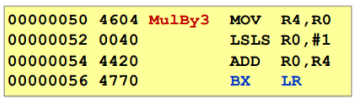
\includegraphics[width=\linewidth]{images/subroutine.png}
\end{minipage}
\begin{minipage}{0.4\linewidth}
in detail:
\begin{itemize}
  \item Label with name \textcolor{darkred}{\textbf{MulBy3}}
  \item Return Statement \textcolor{darkblue}{\textbf{BX LR}}
\end{itemize}
\end{minipage}
\end{example2}

\begin{KR}{Using Subroutines and Stack}
Steps for implementing subroutines:
\begin{enumerate}
  \item Define subroutine entry point with label
  \item Save registers that will be modified
    \begin{itemize}
      \item Use PUSH at start
      \item Include LR if calling other subroutines
    \end{itemize}
  \item Implement subroutine logic
  \item Restore registers in reverse order
    \begin{itemize}
      \item Use POP before return
      \item Can return using POP {..., PC} if LR was saved
    \end{itemize}
  \item Return using BX LR if LR wasn't saved
\end{enumerate}
\end{KR}

\begin{remark}
Important considerations:
\begin{itemize}
  \item Always maintain stack alignment
  \item Match PUSH/POP pairs exactly
  \item Be careful with SP manipulation
  \item Consider nesting depth for stack space
\end{itemize}
\end{remark}

\begin{KR}{Subroutine Implementation}\\
Guidelines for implementing subroutines:

1. Basic subroutine:
\begin{lstlisting}[language=armasm, style=basesmol]
proc_name
    PUSH    {LR}           ; Save return address
    ; Subroutine code
    POP     {PC}           ; Return
\end{lstlisting}

2. With register preservation:
\begin{lstlisting}[language=armasm, style=basesmol]
proc_name
    PUSH    {R4-R7, LR}    ; Save modified registers
    ; Subroutine code using R4-R7
    POP     {R4-R7, PC}    ; Restore and return
\end{lstlisting}

3. With local variables:
\begin{lstlisting}[language=armasm, style=basesmol]
proc_name
    PUSH    {R4, LR}       ; Save registers
    SUB     SP, SP, #8     ; Allocate locals
    ; Use [SP] to [SP, #4] for locals
    ADD     SP, SP, #8     ; Deallocate locals
    POP     {R4, PC}       ; Restore and return
\end{lstlisting}
\end{KR}

\begin{example2}{Nested Subroutine Calls}\\
Example of multiple nested calls with stack manipulation:
\begin{lstlisting}[language=armasm, style=basesmol]
    AREA    progCode, CODE, READONLY
    THUMB
main
    LDR     R1, =0x10203040     ; Initial values
    LDR     R2, =0x50607080
    BL      procA               ; Call procA
    BL      procB               ; Call procB
    B       endless

procA
    PUSH    {R1, R2}            ; Save registers
    LDR     R1, =0xAABBCCDD     ; New values
    LDR     R2, =0xEEFF1020
    POP     {R1, R2}            ; Restore registers
    BX      LR                  ; Return

procB
    PUSH    {R1, R2, LR}        ; Save including LR
    LDR     R1, =0x11223344     ; New values
    LDR     R2, =0x55667788
    BL      procC               ; Call procC
    POP     {R1, R2, PC}        ; Return by popping PC

procC
    PUSH    {R1, R2, LR}        ; Save registers
    LDR     R1, =0x11111111     ; New values
    LDR     R2, =0x22222222
    BL      procD               ; Call procD
    POP     {R1, R2, PC}        ; Return by popping PC
\end{lstlisting}

Stack contents at key points:
\begin{itemize}
  \item After procA PUSH: R1(0x10203040), R2(0x50607080)
  \item After procB PUSH: R1, R2, LR(ret\_addr)
  \item After procC PUSH: R1(0x11223344), R2(0x55667788), LR(ret\_addr)
\end{itemize}
\end{example2}



\subsubsection{Stack}

\begin{definition}{Stack}characteristics:
\begin{itemize}
  \item \textcolor{darkblue}{\textbf{Stack Area}} (Section): Continuous RAM section
  \item \textcolor{darkred}{\textbf{Stack Pointer (SP)}}: R13, points to last written value
  \item \textbf{Direction}: Full-descending (grows toward lower addresses)
  \item \textbf{Alignment}: Word-aligned (4 bytes)
  \item \textbf{Data Size}: 32-bit words only
\end{itemize}

Main operations:
\begin{itemize}
  \item \textcolor{darkgreen}{\textbf{PUSH}}: Decrements SP, then stores words
  \item \textcolor{darkgreen}{\textbf{POP}}: Loads words, then increments SP
\end{itemize}

Stack constraints:
\begin{itemize}
  \item Number of PUSH and POP operations must match
  \item SP must stay between stack-limit and stack-base\\
  $\rightarrow$ \textcolor{darkgreen}{Stack-limit} $\leq$ SP $\leq$ \textcolor{darkpurple}{Stack-base}
\end{itemize}

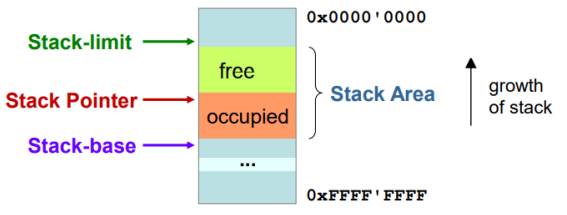
\includegraphics[width=\linewidth]{images/stack_overview.png}


\end{definition}

\begin{concept}{Stack Instructions}
Special stack manipulation instructions:
\vspace{1mm}\\
\begin{minipage}[t]{0.5\linewidth}
\begin{itemize}
  \item \textbf{ADD/SUB SP}:
    \begin{itemize}
      \item Immediate offset 0-508
      \item Must be multiple of 4
    \end{itemize}
  \item \textbf{SP-relative LDR/STR}:
    \begin{itemize}
      \item Immediate offset 0-1020
      \item Used for frame access
    \end{itemize}
\end{itemize}
\end{minipage}
\begin{minipage}[t]{0.5\linewidth}
\begin{itemize}
  \item \textbf{PUSH/POP}:
    \begin{itemize}
      \item Multiple register transfer
      \item Maintains alignment
      \item Can include PC/LR
    \end{itemize}
\end{itemize}
\end{minipage}
\end{concept}



\begin{example2}{PUSH/POP Implementation}

  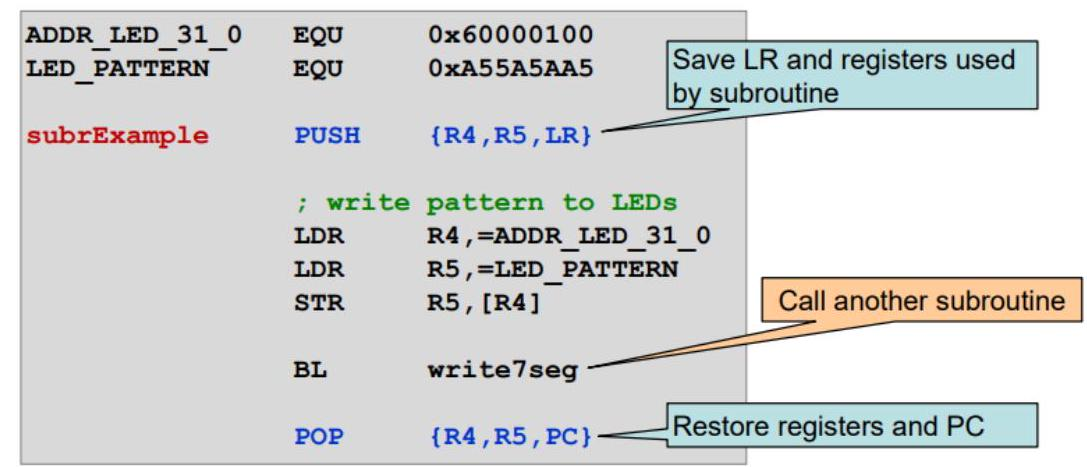
\includegraphics[width=\linewidth]{images/2024_12_29_79e6b22f503fb7b4f718g-08}
\begin{lstlisting}[language=armasm, style=basesmol]
; PUSH {R2,R3,R6}
SUB     SP, SP, #12     ; Reserve stack space
STR     R2, [SP]        ; Store R2
STR     R3, [SP, #4]    ; Store R3
STR     R6, [SP, #8]    ; Store R6

; POP {R2,R3,R6}
LDR     R2, [SP]        ; Restore R2
LDR     R3, [SP, #4]    ; Restore R3
LDR     R6, [SP, #8]    ; Restore R6
ADD     SP, SP, #12     ; Free stack space
\end{lstlisting}
\end{example2}

\subsubsection{Stack Operations and Functions}

\begin{concept}{Stack Operations}
Common stack manipulation patterns:
\begin{itemize}
  \item \textbf{Register Save/Restore}:
    \begin{itemize}
      \item PUSH/POP for callee-saved registers
      \item Multiple register transfer
    \end{itemize}
  \item \textbf{Local Variables}:
    \begin{itemize}
      \item SUB SP to allocate space
      \item Access via SP-relative addressing
      \item ADD SP to deallocate space
    \end{itemize}
  \item \textbf{Return Handling}:
    \begin{itemize}
      \item Save LR if making calls
      \item Return via BX LR or POP \{PC\}
      \item Use PC in POP list when LR saved
    \end{itemize}
\end{itemize}
\end{concept}

\begin{KR}{Function Implementation Patterns}

1. Simple function:
\begin{lstlisting}[language=armasm, style=basesmol]
func    PUSH    {LR}        ; Save return address
        ; Function body
        POP     {PC}        ; Return
\end{lstlisting}

2. Function with locals:
\begin{lstlisting}[language=armasm, style=basesmol]
func    PUSH    {R4, LR}    ; Save registers
        SUB     SP, #8      ; Space for locals
        ; Function body
        ADD     SP, #8      ; Remove locals
        POP     {R4, PC}    ; Return
\end{lstlisting}

3. Function with parameters:
\begin{lstlisting}[language=armasm, style=basesmol]
        ; R0-R3 = first 4 parameters
        ; [SP] = fifth parameter
func    PUSH    {R4-R6, LR} ; Save registers
        LDR     R4, [SP, #16] ; Load 5th param
        ; Function body
        POP     {R4-R6, PC} ; Return
\end{lstlisting}
\end{KR}

\begin{example2}{Stack Frame}
Example of complete function:
\begin{lstlisting}[language=armasm, style=basesmol]
; int calc(int a, int b, int c)
; a in R0, b in R1, c in R2
calc    PUSH    {R4-R6, LR} ; Save registers
        ; Save parameters
        MOVS    R4, R0      ; Save a
        MOVS    R5, R1      ; Save b
        MOVS    R6, R2      ; Save c
        ; Call helper function
        MOVS    R0, R4      ; First param
        BL      helper      ; Call helper
        ; Continue calculation
        ADDS    R0, R5      ; Add b
        ADDS    R0, R6      ; Add c
        
        POP     {R4-R6, PC} ; Return
\end{lstlisting}
\end{example2}

\begin{remark}
Stack usage considerations:
\begin{itemize}
  \item Monitor stack depth in nested calls
  \item Always maintain 8-byte alignment for SP
  \item Consider register usage to minimize stack operations
  \item Be aware of stack space in interrupt handlers
  \item Document stack requirements for functions
\end{itemize}
\end{remark}

\columnbreak

\subsubsection{Stack Frame}

\begin{definition}{Stack Frame Structure}
Components of a stack frame:
\begin{itemize}
  \item \textbf{Saved Registers}:
    \begin{itemize}
      \item Caller-saved (R0-R3, R12)
      \item Callee-saved (R4-R11)
      \item Link register (LR)
    \end{itemize}
  \item \textbf{Local Variables}:
    \begin{itemize}
      \item Allocated on stack if needed
      \item Word-aligned access
    \end{itemize}
  \item \textbf{Parameters}:
    \begin{itemize}
      \item Beyond R0-R3 if needed
      \item Pushed by caller
    \end{itemize}
\end{itemize}

\end{definition}


\begin{KR}{Stack Frame Layout/Management}\\
Steps for function prologue and epilogue, and guidelines for managing stack frames:

1. Frame structure:
\begin{itemize}
  \item Previous stack frame
  \item Return address (LR)
  \item Saved registers
  \item Local variables
  \item Parameters for called functions
\end{itemize}

2. Frame creation/Function prologue:
\begin{lstlisting}[language=armasm, style=basesmol]
    ; Save registers and create frame
    PUSH    {R4-R7, LR}    ; Save registers
    SUB     SP, SP, #frame_size  ; Allocate space
    SUB     SP, SP, #locals ; Allocate local vars
    
    ; Initialize frame if needed
    MOV     R4, #0         ; Clear locals
    STR     R4, [SP, #0]   ; Initialize var1
    STR     R4, [SP, #4]   ; Initialize var2
\end{lstlisting}

3. Stack frame access:
\begin{lstlisting}[language=armasm, style=basesmol]
    ; Access local variables
    LDR     R0, [SP, #offset1]  ; Load local1
    STR     R1, [SP, #offset2]  ; Store to local2

    ; Access parameters
    LDR     R0, [SP, #20]   ; First stack parameter
    ; Access parameters beyond R0-R3
    LDR     R0, [SP, #param_offset] ; Load param
\end{lstlisting}

4. Frame cleanup/Function epilogue:
\begin{lstlisting}[language=armasm, style=basesmol]
    ; Deallocate frame and restore
    ADD     SP, SP, #frame_size  ; Remove locals
    ADD     SP, SP, #locals ; Deallocate locals
    POP     {R4-R7, PC}    ; Restore and return
\end{lstlisting}
\end{KR}

\begin{remark}
Important considerations:
\begin{itemize}
  \item Maintain 8-byte stack alignment
  \item Save LR before any BL instructions
  \item Properly pair PUSH/POP operations
  \item Document stack frame layout
  \item Track stack depth in nested calls
\end{itemize}
\end{remark}



\begin{example2}{Stack Frame Management} Stack frame creation and cleanup:
\begin{lstlisting}[language=armasm, style=basesmol]
func    ; Function prologue
    PUSH    {R4-R8, LR}    ; Save registers
    SUB     SP, SP, #12    ; Allocate locals
    ; Access local variables relative to SP
    STR     R0, [SP, #0]   ; Local var 1
    STR     R1, [SP, #4]   ; Local var 2
    STR     R2, [SP, #8]   ; Local var 3
    ; Function body
    BL      other_func     ; Call another function
    ; Function epilogue
    ADD     SP, SP, #12    ; Deallocate locals
    POP     {R4-R8, PC}    ; Restore and return
\end{lstlisting}
\end{example2}



















	\section{Parameter Passing}

\begin{concept}{Parameter Passing Methods}\\
Data can be passed between functions through:
\begin{itemize}
  \item \textbf{Registers}: Fast, limited number available
  \item \textbf{Global Variables}: Shared memory space
  \item \textbf{Stack}: 
    \begin{itemize}
      \item Caller: PUSH parameters onto stack
      \item Callee: Access via LDR from stack
    \end{itemize}
\end{itemize}
\end{concept}

\begin{definition}{ARM Procedure Call Standard}\\
\textbf{Parameter Passing:}
\begin{itemize}
  \item First four arguments use R0-R3
  \item Additional parameters go on stack
\end{itemize}

\textbf{Return Values:}
\begin{itemize}
  \item \textbf{Small Values} ($\leqslant$ 32 bits): 
    \begin{itemize}
      \item Return in R0
      \item Zero/sign extend if needed
    \end{itemize}
  \item \textbf{Double Word} (64 bits): R0/R1
  \item \textbf{128-bit Values}: R0-R3
  \item \textbf{Larger Values}: 
    \begin{itemize}
      \item Store in memory
      \item Return pointer in R0
    \end{itemize}
\end{itemize}

\textbf{Register Usage:}
\begin{itemize}
  \item \textbf{R0-R3}: Arguments/results (caller-saved)
  \item \textbf{R4-R11}: Local variables (callee-saved)
  \item \textbf{R12}: IP - scratch register
  \item \textbf{R13}: SP - stack pointer
  \item \textbf{R14}: LR - link register
  \item \textbf{R15}: PC - program counter
\end{itemize}

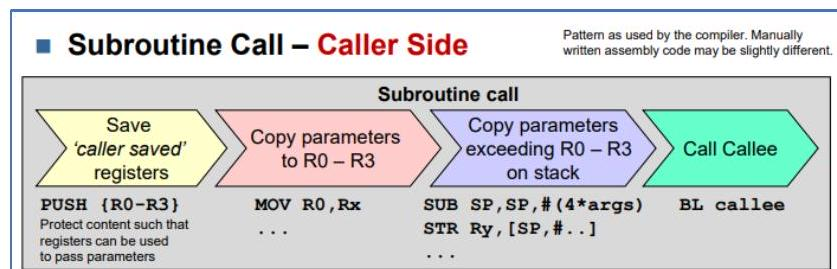
\includegraphics[width=\linewidth]{images/2024_12_29_79e6b22f503fb7b4f718g-09(3)}
\end{definition}

\begin{concept}{Reentrancy}\\
Handling recursive function calls:
\begin{itemize}
  \item Each call needs its own data set
  \item Registers/globals get overwritten
  \item Solution: Use stack for local storage
\end{itemize}
\end{concept}

\begin{example2}{Parameter Passing Methods}
Global variable approach (not recommended):
\begin{lstlisting}[language=armasm, style=basesmol]
    .data
value   DCD     0           ; Global variable

    .text
func    LDR     R0, =value  ; Load address
        LDR     R1, [R0]    ; Get value
        ; Process value
        STR     R1, [R0]    ; Store result
\end{lstlisting}

Register-based approach (preferred):
\begin{lstlisting}[language=armasm, style=basesmol]
func    PUSH    {R4, LR}    ; Save registers
        ; R0 contains input parameter
        MOV     R4, R0      ; Save parameter
        ; Process value in R4
        MOV     R0, R4      ; Set return value
        POP     {R4, PC}    ; Restore and return
\end{lstlisting}
\end{example2}

\begin{KR}{Implementing Function Calls}\\
Steps for calling functions:
\begin{enumerate}
  \item Caller's responsibilities:
    \begin{itemize}
      \item Place parameters in R0-R3
      \item Push additional parameters on stack
      \item Save caller-saved registers if needed
    \end{itemize}
  \item Callee's responsibilities:
    \begin{itemize}
      \item Save callee-saved registers used
      \item Save LR if making other calls
      \item Process parameters
      \item Place return value in R0
      \item Restore saved registers
    \end{itemize}
\end{enumerate}
\end{KR}

\begin{remark}
Important considerations:
\begin{itemize}
  \item Avoid global variables for parameter passing
  \item Use registers for efficiency
  \item Follow ARM calling convention strictly
  \item Consider stack usage in recursive functions
\end{itemize}
\end{remark}

\begin{KR}{Parameter Passing by Value vs. Reference}\\
Two main approaches:
\begin{itemize}
  \item \textbf{Pass by Value}:
    \begin{itemize}
      \item Copies value to function
      \item Changes don't affect original
      \item Default in C
      \item Example: Simple types, integers
    \end{itemize}
  \item \textbf{Pass by Reference}:
    \begin{itemize}
      \item Passes memory address
      \item Changes affect original value
      \item In C: Using pointers
      \item Example: Arrays, large structures
    \end{itemize}
\end{itemize}

Example implementation:
\begin{lstlisting}[language=armasm, style=base]
; Pass by value
func1   PUSH    {LR}
        ADDS    R0, #1      ; Modify parameter
        POP     {PC}        ; Original unchanged

; Pass by reference
func2   PUSH    {LR}
        LDR     R1, [R0]    ; Load from address
        ADDS    R1, #1      ; Modify value
        STR     R1, [R0]    ; Store back to address
        POP     {PC}        ; Original changed
\end{lstlisting}
\end{KR}

\begin{example2}{Data Structure Access}
Working with structures and arrays:
\begin{lstlisting}[language=C, style=base]
typedef struct {
    uint32_t minutes;
    uint32_t seconds;
} time_t;

time_t time;
\end{lstlisting}

Assembly implementation:
\begin{lstlisting}[language=armasm, style=base]
    ; Access structure members
    LDR     R0, =time       ; Get structure address
    LDR     R1, [R0, #0]    ; Load minutes
    LDR     R2, [R0, #4]    ; Load seconds
    
    ; Modify structure
    ADDS    R2, #1          ; Increment seconds
    CMP     R2, #60         ; Check for overflow
    BLT     store_back
    MOVS    R2, #0          ; Reset seconds
    ADDS    R1, #1          ; Increment minutes
store_back
    STR     R1, [R0, #0]    ; Store minutes
    STR     R2, [R0, #4]    ; Store seconds
\end{lstlisting}
\end{example2}

\begin{concept}{Stack Frame Organization}\\
Complete stack frame layout:

\begin{itemize}
  \item \textbf{Previous Stack Frame:}
    \begin{itemize}
      \item Local variables
      \item Saved registers
    \end{itemize}
  \item \textbf{Current Frame:}
    \begin{itemize}
      \item Arguments 5+
      \item Return address (LR)
      \item Saved registers (R4-R11)
      \item Local variables
      \item Temporary storage
    \end{itemize}
  \item \textbf{Next Frame:}
    \begin{itemize}
      \item Space for called functions
    \end{itemize}
\end{itemize}
\end{concept}

\begin{example2}{Recursive Function Implementation}
Factorial calculation:
\begin{lstlisting}[language=armasm, style=base]
; uint32_t factorial(uint32_t n)
; Input in R0, result in R0
factorial
    PUSH    {R4, LR}        ; Save registers
    MOVS    R4, R0          ; Save n
    CMP     R4, #1          ; Check base case
    BLE     fact_end        ; Return 1 if n <= 1
    
    SUBS    R0, R4, #1      ; n-1
    BL      factorial       ; Recursive call
    MULS    R0, R4, R0      ; n * factorial(n-1)
    
fact_end
    POP     {R4, PC}        ; Restore and return
\end{lstlisting}
\end{example2}

\begin{KR}{Function Parameter Guidelines}\\
Best practices for parameter passing:

1. Register Usage:
\begin{itemize}
  \item R0-R3: First four parameters
  \item R0: Return value
  \item R4-R11: Preserve if used
\end{itemize}

2. Stack Usage:
\begin{itemize}
  \item Additional parameters pushed right to left
  \item Maintain 8-byte alignment
  \item Caller responsible for cleaning up stack
\end{itemize}

3. Memory Structures:
\begin{itemize}
  \item Pass pointers for large structures
  \item Use registers for small values
  \item Consider alignment requirements
\end{itemize}

Example implementation:
\begin{lstlisting}[language=armasm, style=base]
; void func(int a, int b, int c, int d, int e)
; First four params in R0-R3, fifth on stack
func    PUSH    {R4-R6, LR} ; Save registers
        
        ; Save parameters
        MOV     R4, R0      ; Save a
        MOV     R5, R1      ; Save b
        MOV     R6, R2      ; Save c
        ; R3 contains d
        LDR     R0, [SP, #16] ; Load e from stack
        
        ; Function body
        
        POP     {R4-R6, PC} ; Return
\end{lstlisting}
\end{KR}

\begin{example2}{Complex Parameter Example}
Function with mixed parameter types:
\begin{lstlisting}[language=C, style=base]
typedef struct {
    int32_t x;
    int32_t y;
} point_t;

int32_t calculate(point_t* p, int32_t scale, 
                  int32_t* result);
\end{lstlisting}

Assembly implementation:
\begin{lstlisting}[language=armasm, style=base]
; R0 = point_t* p
; R1 = scale
; R2 = result pointer
calculate
    PUSH    {R4-R5, LR}     ; Save registers
    
    ; Load structure members
    LDR     R4, [R0, #0]    ; Load p->x
    LDR     R5, [R0, #4]    ; Load p->y
    
    ; Perform calculation
    MULS    R4, R1, R4      ; x * scale
    MULS    R5, R1, R5      ; y * scale
    
    ; Store result
    STR     R4, [R2, #0]    ; *result = x
    ADDS    R0, R4, R5      ; Return sum
    
    POP     {R4-R5, PC}     ; Return
\end{lstlisting}
\end{example2}
	\section{Modular Coding and Linking}

\begin{concept}{Modular Programming Overview}\\
Program code is divided into modules with:
\begin{itemize}
  \item Each source file compiled into separate object file
  \item All object files linked into single executable
  \item Clear interfaces between modules
\end{itemize}

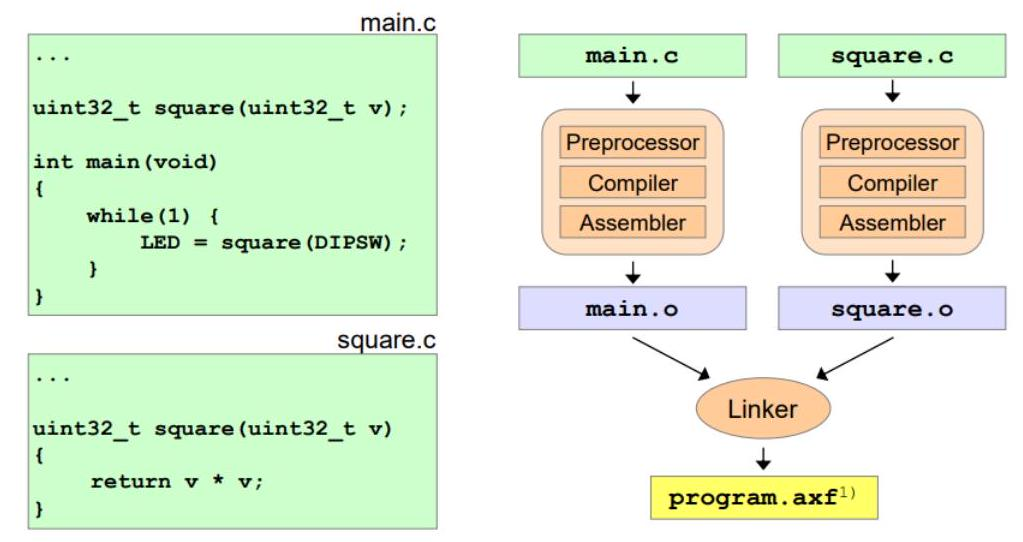
\includegraphics[width=\linewidth]{images/2024_12_29_79e6b22f503fb7b4f718g-10(2)}
\end{concept}

\begin{definition}{Benefits of Modular Programming}\\
Key advantages:
\begin{itemize}
  \item \textbf{Team Development}:
    \begin{itemize}
      \item Multiple developers working on same codebase
      \item Clear ownership of modules
    \end{itemize}
  \item \textbf{Code Organization}:
    \begin{itemize}
      \item Logical partitioning of functionality
      \item Easier code reuse
    \end{itemize}
  \item \textbf{Development Efficiency}:
    \begin{itemize}
      \item Individual module testing
      \item Faster compilation (only changed modules)
      \item Reusable library creation
    \end{itemize}
  \item \textbf{Language Integration}:
    \begin{itemize}
      \item Mix C and assembly modules
      \item Language-specific optimizations
    \end{itemize}
\end{itemize}
\end{definition}

\begin{definition}{Module Linkage}\\
Keywords for controlling module interfaces:
\begin{itemize}
  \item \textbf{EXPORT}: Make symbol available to other modules
  \item \textbf{IMPORT}: Use symbol from another module
  \item Internal symbols: Neither IMPORT nor EXPORT
\end{itemize}

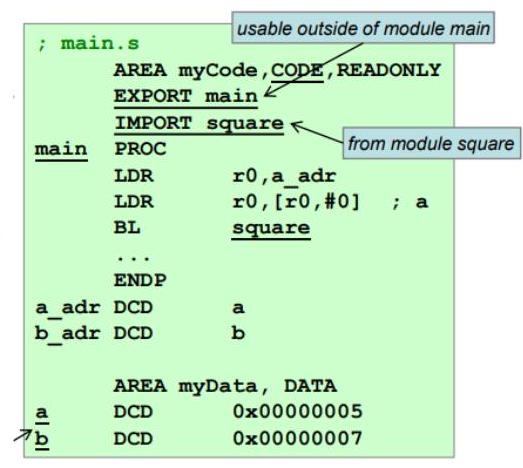
\includegraphics[width=\linewidth]{images/2024_12_29_79e6b22f503fb7b4f718g-10(1)}
\end{definition}

\begin{definition}{Object Files}\\
ELF format contains:
\begin{itemize}
  \item \textbf{Code Section}:
    \begin{itemize}
      \item Program code and constants
      \item Based at address 0x0
    \end{itemize}
  \item \textbf{Data Section}:
    \begin{itemize}
      \item Global variables
      \item Based at address 0x0
    \end{itemize}
  \item \textbf{Symbol Table}:
    \begin{itemize}
      \item All symbols and their attributes
      \item Global/local status
      \item References to external symbols
    \end{itemize}
  \item \textbf{Relocation Table}:
    \begin{itemize}
      \item Instructions for adjusting addresses
      \item Applied during linking process
    \end{itemize}
\end{itemize}
\end{definition}

\begin{concept}{Linker Operation}\\
Main tasks:
\begin{itemize}
  \item Merge code sections from all objects
  \item Merge data sections from all objects
  \item Resolve symbol references between modules
  \item Relocate addresses to final positions
\end{itemize}

Output is ARM Executable File (AXF):

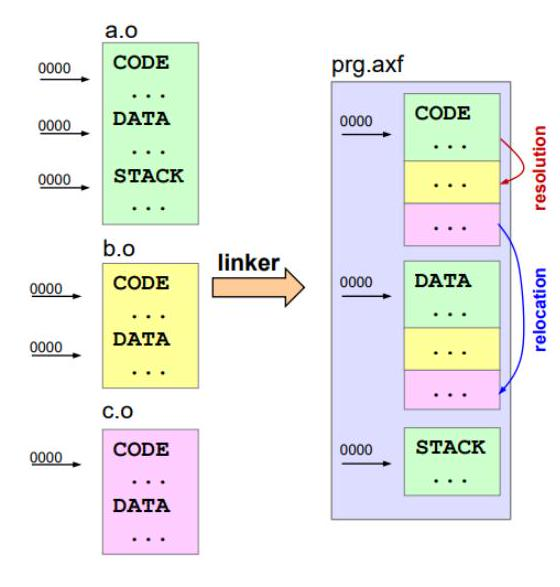
\includegraphics[width=\linewidth]{images/2024_12_29_79e6b22f503fb7b4f718g-10}
\end{concept}

\begin{example2}{Module Interface Example}
\begin{lstlisting}[language=armasm, style=basesmol]
    ; Module A - Defining function
    AREA myCode, CODE, READONLY
    EXPORT myFunction    ; Make available externally
myFunction
    PUSH    {LR}
    ; function code here
    POP     {PC}
    
    ; Module B - Using function
    AREA myCode, CODE, READONLY
    IMPORT myFunction    ; Use external function
    
    BL      myFunction   ; Call the function
\end{lstlisting}
\end{example2}

\begin{KR}{Creating Modular Programs}\\
Steps for modular development:
\begin{enumerate}
  \item Design module structure:
    \begin{itemize}
      \item Identify clear boundaries
      \item Define interfaces
    \end{itemize}
  \item Create individual modules:
    \begin{itemize}
      \item Declare IMPORT/EXPORT
      \item Implement functionality
    \end{itemize}
  \item Compile modules separately
  \item Link modules:
    \begin{itemize}
      \item Resolve references
      \item Create executable
    \end{itemize}
  \item Test integrated system
\end{enumerate}
\end{KR}
	\section{Exceptional Control Flow}

\begin{concept}{Exception Types}\\
Two main categories of exceptions:

\textbf{Interrupt Sources:}
\begin{itemize}
  \item Peripherals requesting immediate CPU attention
  \item Software-generated interrupts
  \item Asynchronous to instruction execution
\end{itemize}

\textbf{System Exceptions:}
\begin{itemize}
  \item \textbf{Reset}: Processor restart
  \item \textbf{NMI}: Non-maskable Interrupt (cannot be ignored)
  \item \textbf{Faults}: Undefined instructions, errors
  \item \textbf{System Calls}: OS services (SVC and PendSV)
\end{itemize}
\end{concept}

\begin{definition}{Interrupt Control}\\
PRIMASK register controls interrupt handling:
\begin{itemize}
  \item Single bit controls all maskable interrupts
  \item Reset state: PRIMASK = 0 (interrupts enabled)
  \item Control methods:
    \begin{itemize}
      \item Assembly: \texttt{CPSID i} (disable), \texttt{CPSIE i} (enable)
      \item C: \texttt{\_\_disable\_irq()}, \texttt{\_\_enable\_irq()}
    \end{itemize}
\end{itemize}

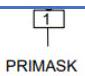
\includegraphics[width=\linewidth]{images/2024_12_29_79e6b22f503fb7b4f718g-11}
\end{definition}

\begin{definition}{Context Storage}\\
Interrupt handling requires automatic context saving:

\textbf{ISR Entry:}
\begin{itemize}
  \item Stores on stack:
    \begin{itemize}
      \item xPSR, PC, LR, R12
      \item R0-R3 (caller-saved registers)
    \end{itemize}
  \item Stores EXC\_RETURN in LR
\end{itemize}

\textbf{ISR Exit:}
\begin{itemize}
  \item Via BX LR or POP {..., PC}
  \item Restores from stack:
    \begin{itemize}
      \item R0-R3, R12, LR, PC
      \item xPSR
    \end{itemize}
\end{itemize}
\end{definition}

\begin{concept}{Polling vs Interrupts}\\
\textbf{Polling Approach:}
\begin{itemize}
  \item Periodic status register checks
  \item Synchronous with main program
  \item \textbf{Advantages:}
    \begin{itemize}
      \item Simple implementation
      \item Predictable timing
      \item No extra hardware needed
    \end{itemize}
  \item \textbf{Disadvantages:}
    \begin{itemize}
      \item CPU wastes time waiting
      \item Reduced system throughput
      \item Longer response times
    \end{itemize}
\end{itemize}

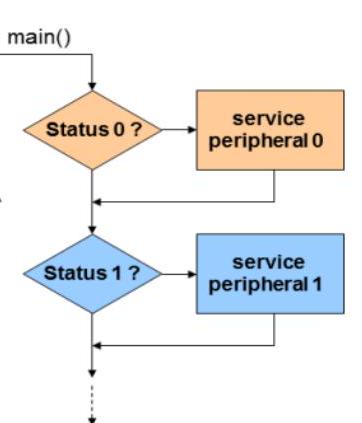
\includegraphics[width=\linewidth]{images/2024_12_29_79e6b22f503fb7b4f718g-11(1)}

\textbf{Interrupt Approach:}
\begin{itemize}
  \item Hardware-triggered event handling
  \item Asynchronous to main program
  \item \textbf{Advantages:}
    \begin{itemize}
      \item Efficient CPU usage
      \item Quick response times
      \item Better system throughput
    \end{itemize}
  \item \textbf{Disadvantages:}
    \begin{itemize}
      \item More complex implementation
      \item Harder to debug
      \item Timing less predictable
    \end{itemize}
\end{itemize}

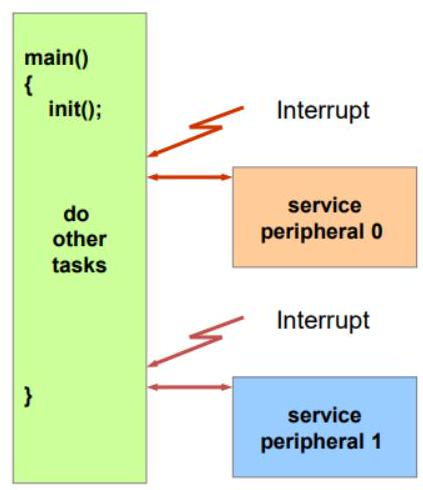
\includegraphics[width=\linewidth]{images/2024_12_29_79e6b22f503fb7b4f718g-11(2)}
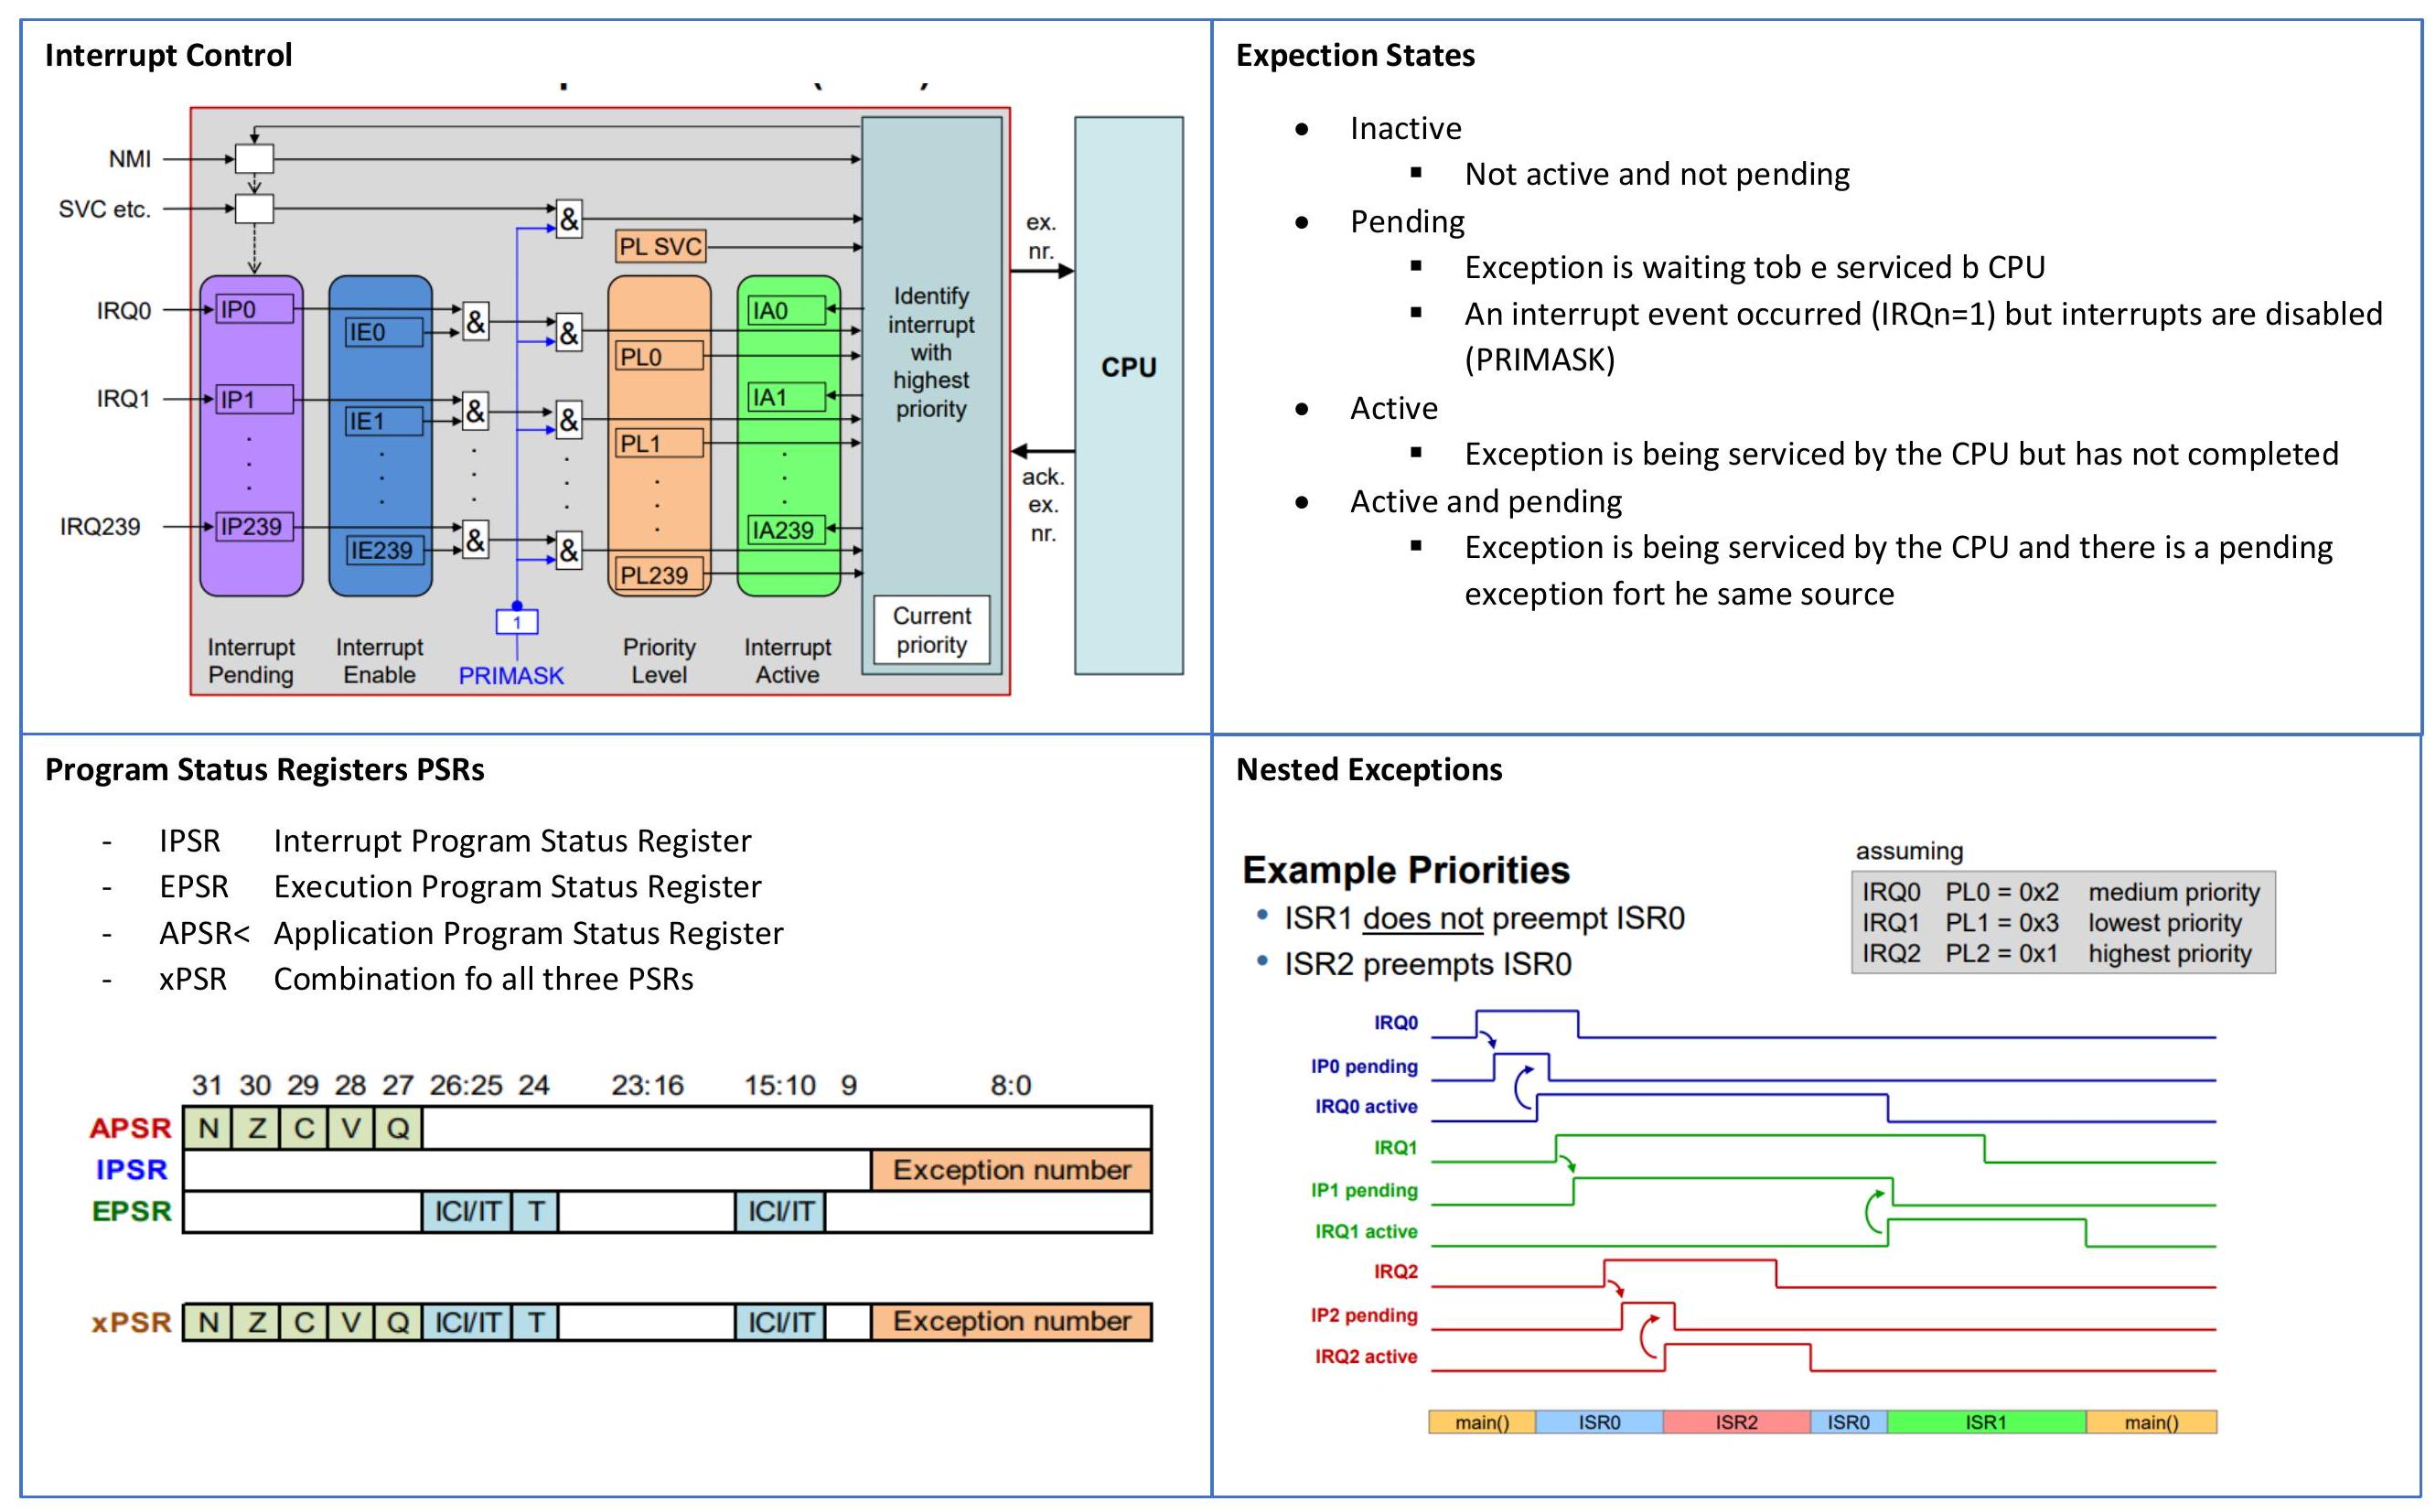
\includegraphics[width=\linewidth]{images/2024_12_29_79e6b22f503fb7b4f718g-12}
\end{concept}

\begin{example2}{Basic ISR Implementation}
\begin{lstlisting}[language=armasm, style=basesmol]
    ; Interrupt Service Routine
    EXPORT MyISR
MyISR
    PUSH    {R4-R7, LR}    ; Save registers
    
    ; Handle interrupt here
    ; R0-R3 already saved automatically
    
    POP     {R4-R7, PC}    ; Restore and return
\end{lstlisting}
\end{example2}

\begin{KR}{Implementing Interrupt Handlers}\\
Steps for implementing interrupt handlers:
\begin{enumerate}
  \item Define interrupt vector
  \item Save necessary context
  \item Handle the interrupt
  \item Clear interrupt flag
  \item Restore context
  \item Return from interrupt
\end{enumerate}

Important considerations:
\begin{itemize}
  \item Keep ISRs short
  \item Handle critical tasks only
  \item Be aware of nested interrupts
  \item Protect shared resources
\end{itemize}
\end{KR}

\begin{concept}{NVIC (Nested Vectored Interrupt Controller)}\\
Key components and functionality:
\begin{itemize}
  \item \textbf{Interrupt States}:
    \begin{itemize}
      \item \textbf{Inactive}: Not active and not pending
      \item \textbf{Pending}: Waiting to be serviced
      \item \textbf{Active}: Currently being serviced
      \item \textbf{Active and Pending}: Being serviced with new request
    \end{itemize}
  \item \textbf{Control Registers}:
    \begin{itemize}
      \item Interrupt Enable (IE)
      \item Interrupt Pending (IP)
      \item Interrupt Active (IA)
      \item Priority Level (PL)
    \end{itemize}
\end{itemize}

%\includegraphics[width=\linewidth]{images/2024_12_29_79e6b22f503fb7b4f718g-11(3)}
\end{concept}

\begin{formula}{Interrupt Control Registers}\\
Important NVIC registers:

1. Enable/Disable Registers:
\begin{lstlisting}[language=armasm, style=base]
SETENA0 EQU 0xE000E100    ; Enable interrupts
CLRENA0 EQU 0xE000E180    ; Disable interrupts

; Enable IRQ3
LDR     R0, =SETENA0
MOVS    R1, #(1<<3)
STR     R1, [R0]

; Disable IRQ3
LDR     R0, =CLRENA0
MOVS    R1, #(1<<3)
STR     R1, [R0]
\end{lstlisting}

2. Pending Registers:
\begin{lstlisting}[language=armasm, style=base]
SETPEND0 EQU 0xE000E200   ; Set pending
CLRPEND0 EQU 0xE000E280   ; Clear pending

; Set IRQ3 pending
LDR     R0, =SETPEND0
MOVS    R1, #(1<<3)
STR     R1, [R0]

; Clear IRQ3 pending
LDR     R0, =CLRPEND0
MOVS    R1, #(1<<3)
STR     R1, [R0]
\end{lstlisting}
\end{formula}

\begin{concept}{Priority System}\\
Interrupt priority handling:
\begin{itemize}
  \item \textbf{Priority Levels}:
    \begin{itemize}
      \item 0-255 (lower number = higher priority)
      \item Fixed priorities for system exceptions
      \item Programmable priorities for IRQs
    \end{itemize}
  \item \textbf{Preemption}:
    \begin{itemize}
      \item Higher priority interrupts can preempt lower
      \item Same priority follows FIFO
    \end{itemize}
\end{itemize}

Example priority setting:
\begin{lstlisting}[language=C, style=base]
// Set priority for IRQ3
NVIC_SetPriority(IRQ3_IRQn, 2);

// Get priority
uint32_t prio = NVIC_GetPriority(IRQ3_IRQn);
\end{lstlisting}
\end{concept}

\begin{KR}{Exception Vector Table}\\
Setup and usage:

1. Vector table structure:
\begin{lstlisting}[language=armasm, style=base]
    AREA RESET, DATA, READONLY
__Vectors
    DCD     __initial_sp        ; Top of Stack
    DCD     Reset_Handler       ; Reset
    DCD     NMI_Handler        ; NMI
    DCD     HardFault_Handler  ; Hard Fault
    DCD     0                  ; Reserved
    DCD     0                  ; Reserved
    DCD     0                  ; Reserved
    ; ... more vectors
    DCD     IRQ0_Handler       ; IRQ0
    DCD     IRQ1_Handler       ; IRQ1
\end{lstlisting}

2. Handler implementation:
\begin{lstlisting}[language=armasm, style=base]
    AREA |.text|, CODE, READONLY
    
IRQ0_Handler PROC
    EXPORT IRQ0_Handler
    PUSH    {R4-R7,LR}
    ; Handle interrupt
    POP     {R4-R7,PC}
    ENDP
\end{lstlisting}
\end{KR}

\begin{example2}{Nested Interrupts Example}
Implementation with different priorities:
\begin{lstlisting}[language=C, style=base]
// Initialize interrupts
void init_interrupts(void) {
    // Enable interrupts
    NVIC_EnableIRQ(IRQ0_IRQn);
    NVIC_EnableIRQ(IRQ1_IRQn);
    
    // Set priorities
    NVIC_SetPriority(IRQ0_IRQn, 1); // Higher
    NVIC_SetPriority(IRQ1_IRQn, 2); // Lower
    
    // Enable global interrupts
    __enable_irq();
}

// Higher priority ISR
void IRQ0_Handler(void) {
    // Handle high priority interrupt
    // Can't be interrupted by IRQ1
}

// Lower priority ISR
void IRQ1_Handler(void) {
    // Handle low priority interrupt
    // Can be interrupted by IRQ0
}
\end{lstlisting}
\end{example2}

\begin{concept}{Data Consistency}\\
Handling shared data access:
\begin{itemize}
  \item \textbf{Race Conditions}:
    \begin{itemize}
      \item Main program and ISR accessing same data
      \item Interrupts during multi-step operations
    \end{itemize}
  \item \textbf{Solutions}:
    \begin{itemize}
      \item Disable interrupts during critical sections
      \item Use atomic operations
      \item Implement proper synchronization
    \end{itemize}
\end{itemize}

Example protection:
\begin{lstlisting}[language=C, style=base]
void update_shared_data(void) {
    __disable_irq();         // Critical section start
    shared_var++;           // Update shared data
    __enable_irq();         // Critical section end
}
\end{lstlisting}
\end{concept}

\begin{KR}{CMSIS Functions for Interrupt Control}\\
Standard CMSIS functions for interrupt handling:
\begin{itemize}
  \item \texttt{NVIC\_EnableIRQ(IRQn)}: Enable specific interrupt
  \item \texttt{NVIC\_DisableIRQ(IRQn)}: Disable specific interrupt
  \item \texttt{NVIC\_SetPendingIRQ(IRQn)}: Set interrupt pending
  \item \texttt{NVIC\_ClearPendingIRQ(IRQn)}: Clear pending status
  \item \texttt{NVIC\_SetPriority(IRQn, priority)}: Set priority
  \item \texttt{NVIC\_GetPriority(IRQn)}: Read priority
\end{itemize}

Example usage:
\begin{lstlisting}[language=C, style=base]
void init_timer_interrupt(void) {
    // Enable timer interrupt
    NVIC_EnableIRQ(TIM2_IRQn);
    
    // Set priority
    NVIC_SetPriority(TIM2_IRQn, 2);
    
    // Configure timer
    // ...
    
    // Enable global interrupts
    __enable_irq();
}
\end{lstlisting}
\end{KR}
	\section{Increasing System Performance}

\begin{concept}{Performance Optimization Trade-offs}\\
\begin{tabular}{|l|l|}
\hline
\textbf{Optimizing for} & \textbf{Drawbacks on} \\
\hline
Higher speed & Power, cost, chip area \\
\hline
Lower cost & Speed, reliability \\
\hline
Zero power consumption & Speed, cost \\
\hline
Super reliable & Chip area, cost, speed \\
\hline
Temperature range & Power, cost, lifetime \\
\hline
\end{tabular}
\end{concept}

\begin{concept}{Instruction Set Architectures}\\
\textbf{RISC (Reduced Instruction Set Computer):}
\begin{itemize}
  \item Few instructions with uniform format
  \item Fast decoding, simple addressing
  \item Less hardware → higher clock rates
  \item More chip space for registers (up to 256)
  \item Load-store architecture reduces memory access
  \item CPU works at full speed on registers
  \item Enables shorter, efficient pipelines 
\end{itemize}

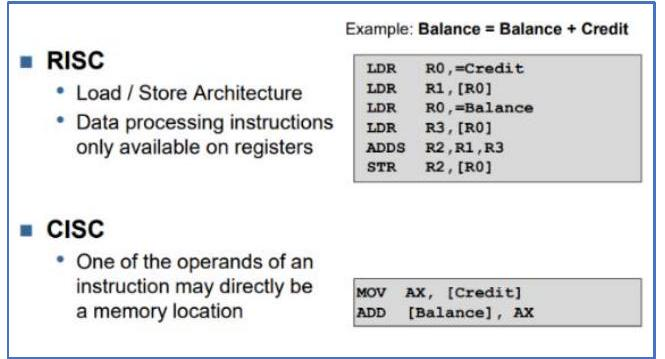
\includegraphics[width=\linewidth]{images/2024_12_29_79e6b22f503fb7b4f718g-13(1)}

\textbf{CISC (Complex Instruction Set Computer):}
\begin{itemize}
  \item More complex instruction set
  \item Lower memory usage for programs
  \item Potential performance gain for short programs
  \item More complex hardware required
\end{itemize}
\end{concept}

\begin{definition}{Computer Architectures}\\
\textbf{Von Neumann Architecture:}
\begin{itemize}
  \item Single memory for program and data
  \item Single bus system between CPU and memory
\end{itemize}

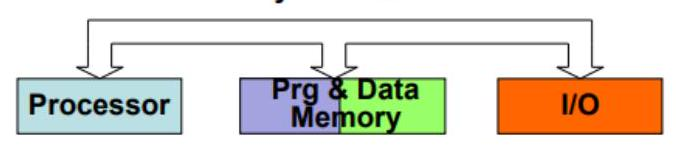
\includegraphics[width=\linewidth]{images/2024_12_29_79e6b22f503fb7b4f718g-13}

\textbf{Harvard Architecture:}
\begin{itemize}
  \item Separate program and data memories
  \item Two sets of address/data buses
  \item Originally from Harvard Mark I
\end{itemize}

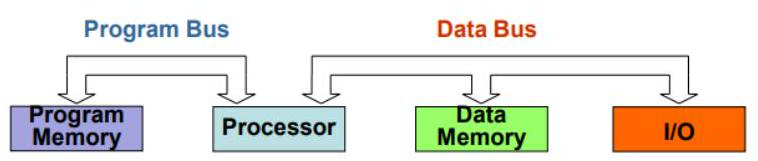
\includegraphics[width=\linewidth]{images/2024_12_29_79e6b22f503fb7b4f718g-13(2)}
\end{definition}

\begin{concept}{Pipelining}\\
Process of fetching next instruction while current one decodes:

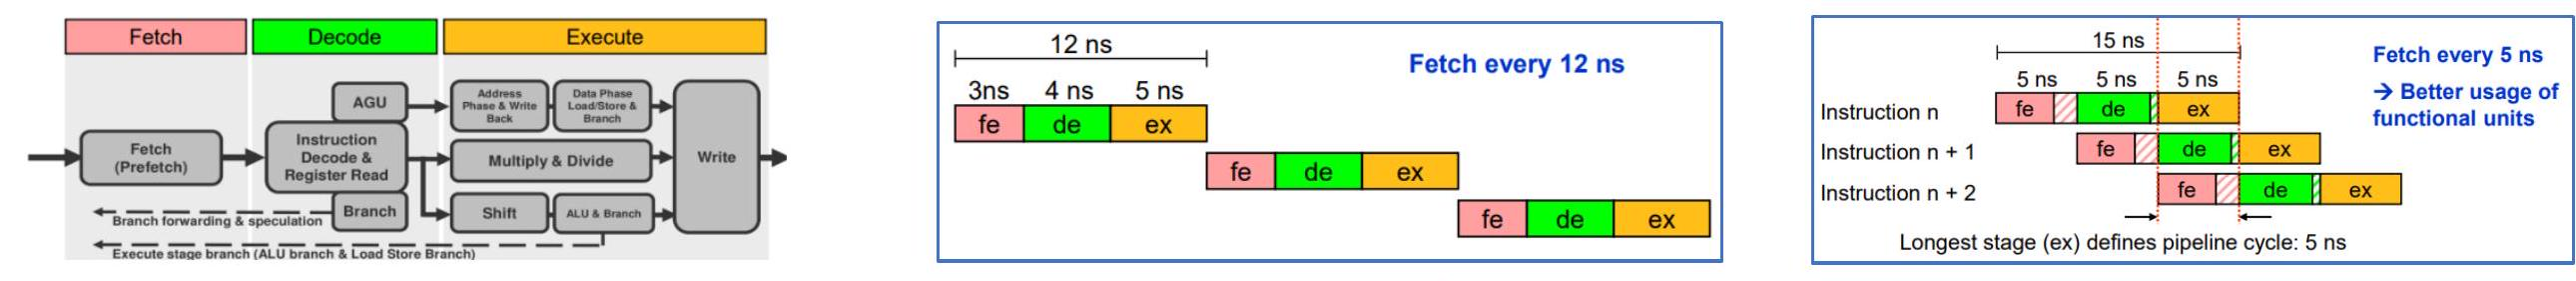
\includegraphics[width=\linewidth]{images/2024_12_29_79e6b22f503fb7b4f718g-14(2)}

\textbf{Pipeline Stages (Example):}
\begin{itemize}
  \item Fetch (Fe): Read instruction - 3ns
  \item Decode (De): Process instruction - 4ns
  \item Execute (Ex): Execute and writeback - 5ns
\end{itemize}

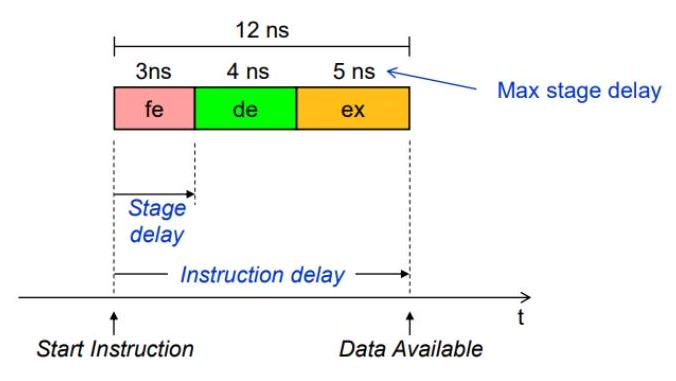
\includegraphics[width=\linewidth]{images/2024_12_29_79e6b22f503fb7b4f718g-14(1)}

\textbf{Advantages:}
\begin{itemize}
  \item Uniform execution time per stage
  \item Significant performance improvement
  \item Simpler hardware per stage
\end{itemize}

\textbf{Disadvantages:}
\begin{itemize}
  \item Blocking stages affect whole pipeline
  \item Memory access conflicts between stages
\end{itemize}
\end{concept}

\begin{definition}{Pipeline Performance}\\
Without pipelining:
\[\frac{\text{Instructions}}{\text{second}} = \frac{1}{\text{Instruction delay}}\]

With pipelining:
\[\frac{\text{Instructions}}{\text{second}} = \frac{1}{\text{Max stage delay}}\]

Note: Pipeline must be filled first
\end{definition}

\begin{example2}{Pipeline Execution}\\
\textbf{Optimal Case:}
\begin{itemize}
  \item Register-only operations
  \item 6 instructions in 6 cycles
  \item CPI = 1 (Cycles Per Instruction)
\end{itemize}

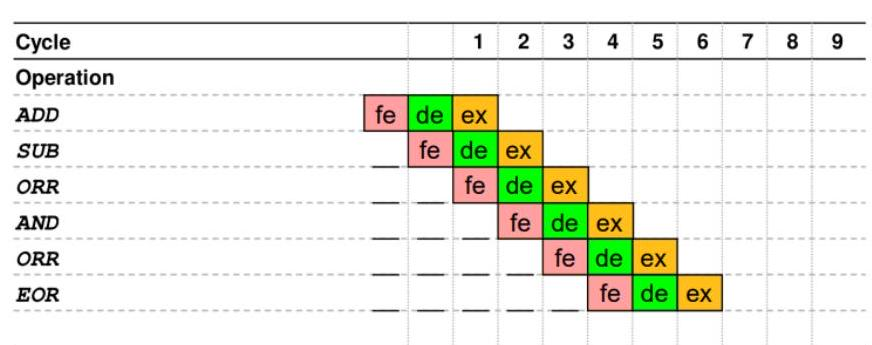
\includegraphics[width=\linewidth]{images/2024_12_29_79e6b22f503fb7b4f718g-14}

\textbf{LDR Special Case:}
\begin{itemize}
  \item 6 instructions in 7 cycles due to memory access
  \item Pipeline stalls for memory read
  \item CPI = 1.2
\end{itemize}
\end{example2}

\begin{concept}{Pipeline Hazards and Optimization}\\
\textbf{Control Hazards:}
\begin{itemize}
  \item Branch decisions in execute stage
  \item Pipeline stalls for taken branches
\end{itemize}

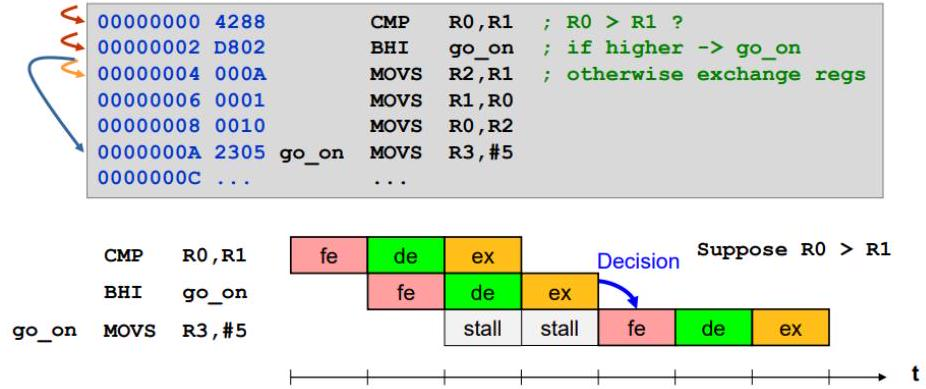
\includegraphics[width=\linewidth]{images/2024_12_29_79e6b22f503fb7b4f718g-15}

\textbf{Optimization Techniques:}
\begin{itemize}
  \item Branch prediction based on history
  \item Instruction prefetch
  \item Out-of-order execution
\end{itemize}

\textbf{Optimization Limits:}
\begin{itemize}
  \item Security vulnerabilities (Meltdown, Spectre)
  \item Complex optimizations increase risk
\end{itemize}
\end{concept}

\begin{concept}{Parallel Computing}\\
Different approaches to parallelism:
\begin{itemize}
  \item \textbf{Vector Processing}: Single instruction processes multiple data
  \item \textbf{Multithreading}: Multiple threads share CPU
  \item \textbf{Multicore}: Multiple CPU cores on one chip
  \item \textbf{Multiprocessor}: Multiple CPUs in system
\end{itemize}
\end{concept}

\begin{KR}{Optimizing System Performance}\\
Steps for performance optimization:
\begin{enumerate}
  \item Analyze performance bottlenecks
  \item Choose appropriate architecture:
    \begin{itemize}
      \item RISC vs CISC based on application
      \item Consider memory architecture
    \end{itemize}
  \item Implement pipelining:
    \begin{itemize}
      \item Balance stage delays
      \item Handle hazards appropriately
    \end{itemize}
  \item Consider parallelization options
  \item Evaluate security implications
\end{enumerate}
\end{KR}

\begin{concept}{Performance Growth Overview}\\
Historical development:
\begin{itemize}
  \item Early improvements:
    \begin{itemize}
      \item Increasing clock frequencies
      \item Better manufacturing processes
      \item Smaller transistor sizes
    \end{itemize}
  \item Modern improvements:
    \begin{itemize}
      \item Advanced architectural concepts (RISC, Pipelining)
      \item Multiple cores
      \item Specialized hardware units
    \end{itemize}
  \item Current limitations:
    \begin{itemize}
      \item Power density
      \item Heat dissipation
      \item Memory wall
      \item Parallelization overhead
    \end{itemize}
\end{itemize}
\end{concept}

\begin{concept}{System Level Optimization}\\
Different approaches to improve performance:
\begin{itemize}
  \item \textbf{External Factors}:
    \begin{itemize}
      \item Better compiler optimization
      \item Improved algorithms
      \item Efficient software design
    \end{itemize}
  \item \textbf{System Level Factors}:
    \begin{itemize}
      \item Special Purpose Units (e.g., Crypto, Video)
      \item Multiple Processors
      \item Bus Architecture optimization
      \item Faster peripheral components
    \end{itemize}
  \item \textbf{CPU Improvements}:
    \begin{itemize}
      \item Increased Clock Speed
      \item Cache Memory
      \item Multiple Cores
      \item Pipeline Optimization
      \item Branch Prediction
      \item Out-of-Order Execution
    \end{itemize}
\end{itemize}
\end{concept}

\begin{formula}{Pipeline Performance Calculation}\\
For a processor with n pipeline stages:

\textbf{Without pipelining:}
\begin{itemize}
  \item Time per instruction = Sum of all stage delays
  \item Performance = $\frac{1}{\text{Total delay}}$
\end{itemize}

\textbf{With pipelining:}
\begin{itemize}
  \item Time per instruction = Longest stage delay
  \item Initial latency = n cycles
  \item Throughput = $\frac{1}{\text{Max stage delay}}$
\end{itemize}

Example calculation:
\begin{itemize}
  \item Stage delays: Fe=3ns, De=4ns, Ex=5ns
  \item Without pipeline: 12ns per instruction
  \item With pipeline: 5ns per instruction after filling
  \item Performance improvement: 2.4×
\end{itemize}
\end{formula}

\begin{example2}{Pipeline Hazards}
Three types of pipeline hazards:

1. \textbf{Structural Hazards}:
\begin{lstlisting}[style=base]
LDR  R0, [R1]    ; Needs memory access
LDR  R2, [R3]    ; Also needs memory access
; Memory system can't handle both at once
\end{lstlisting}

2. \textbf{Data Hazards}:
\begin{lstlisting}[style=base]
ADDS R0, R1, R2  ; R0 gets new value
ADDS R3, R0, R4  ; Uses R0 before ready
; Second instruction must wait
\end{lstlisting}

3. \textbf{Control Hazards}:
\begin{lstlisting}[style=base]
CMP  R0, #0      ; Compare
BEQ  target      ; Branch if equal
ADD  R1, R2, R3  ; May be unnecessary
SUB  R4, R5, R6  ; May be unnecessary
target
; Pipeline must flush if branch taken
\end{lstlisting}
\end{example2}

\begin{concept}{Parallel Processing Models}\\
\textbf{SISD (Single Instruction Single Data):}
\begin{itemize}
  \item Traditional sequential processing
  \item One instruction processes one data item
  \item Example: Basic scalar processor
\end{itemize}

\textbf{SIMD (Single Instruction Multiple Data):}
\begin{itemize}
  \item Vector processing
  \item One instruction processes multiple data items
  \item Examples: MMX, SSE, AVX instructions
\end{itemize}

\textbf{MIMD (Multiple Instruction Multiple Data):}
\begin{itemize}
  \item True parallel processing
  \item Multiple processors execute different instructions
  \item Example: Multicore systems
\end{itemize}
\end{concept}

\begin{KR}{Performance Optimization Guidelines}\\
Steps for system optimization:

1. \textbf{Analyze Requirements}:
\begin{itemize}
  \item Performance targets
  \item Power constraints
  \item Cost limitations
  \item Reliability needs
\end{itemize}

2. \textbf{Choose Architecture}:
\begin{itemize}
  \item RISC vs CISC
  \item Memory architecture
  \item Pipeline depth
  \item Parallelization approach
\end{itemize}

3. \textbf{Optimize Implementation}:
\begin{itemize}
  \item Balance pipeline stages
  \item Implement hazard handling
  \item Consider branch prediction
  \item Optimize memory access
\end{itemize}

4. \textbf{Security Considerations}:
\begin{itemize}
  \item Evaluate optimization risks
  \item Consider side-channel attacks
  \item Balance performance and security
\end{itemize}
\end{KR}

\begin{example2}{Multicore vs Multiprocessor}
Key differences:
\begin{itemize}
  \item \textbf{Multicore}:
    \begin{itemize}
      \item Multiple CPU cores on single chip
      \item Shared cache and memory interface
      \item Lower communication overhead
      \item More power efficient
    \end{itemize}
  \item \textbf{Multiprocessor}:
    \begin{itemize}
      \item Multiple separate CPU chips
      \item Independent caches
      \item Higher communication overhead
      \item More scalable for large systems
    \end{itemize}
\end{itemize}
\end{example2}

\begin{concept}{Performance Growth Overview}\\
Historical development:
\begin{itemize}
  \item Early improvements:
    \begin{itemize}
      \item Increasing clock frequencies
      \item Better manufacturing processes
      \item Smaller transistor sizes
    \end{itemize}
  \item Modern improvements:
    \begin{itemize}
      \item Advanced architectural concepts (RISC, Pipelining)
      \item Multiple cores
      \item Specialized hardware units
    \end{itemize}
  \item Current limitations:
    \begin{itemize}
      \item Power density
      \item Heat dissipation
      \item Memory wall
      \item Parallelization overhead
    \end{itemize}
\end{itemize}
\end{concept}

\begin{concept}{System Level Optimization}\\
Different approaches to improve performance:
\begin{itemize}
  \item \textbf{External Factors}:
    \begin{itemize}
      \item Better compiler optimization
      \item Improved algorithms
      \item Efficient software design
    \end{itemize}
  \item \textbf{System Level Factors}:
    \begin{itemize}
      \item Special Purpose Units (e.g., Crypto, Video)
      \item Multiple Processors
      \item Bus Architecture optimization
      \item Faster peripheral components
    \end{itemize}
  \item \textbf{CPU Improvements}:
    \begin{itemize}
      \item Increased Clock Speed
      \item Cache Memory
      \item Multiple Cores
      \item Pipeline Optimization
      \item Branch Prediction
      \item Out-of-Order Execution
    \end{itemize}
\end{itemize}
\end{concept}

\begin{formula}{Pipeline Performance Calculation}\\
For a processor with n pipeline stages:

\textbf{Without pipelining:}
\begin{itemize}
  \item Time per instruction = Sum of all stage delays
  \item Performance = $\frac{1}{\text{Total delay}}$
\end{itemize}

\textbf{With pipelining:}
\begin{itemize}
  \item Time per instruction = Longest stage delay
  \item Initial latency = n cycles
  \item Throughput = $\frac{1}{\text{Max stage delay}}$
\end{itemize}

Example calculation:
\begin{itemize}
  \item Stage delays: Fe=3ns, De=4ns, Ex=5ns
  \item Without pipeline: 12ns per instruction
  \item With pipeline: 5ns per instruction after filling
  \item Performance improvement: 2.4×
\end{itemize}
\end{formula}

\begin{example2}{Pipeline Hazards}
Three types of pipeline hazards:

1. \textbf{Structural Hazards}:
\begin{lstlisting}[style=base]
LDR  R0, [R1]    ; Needs memory access
LDR  R2, [R3]    ; Also needs memory access
; Memory system can't handle both at once
\end{lstlisting}

2. \textbf{Data Hazards}:
\begin{lstlisting}[style=base]
ADDS R0, R1, R2  ; R0 gets new value
ADDS R3, R0, R4  ; Uses R0 before ready
; Second instruction must wait
\end{lstlisting}

3. \textbf{Control Hazards}:
\begin{lstlisting}[style=base]
CMP  R0, #0      ; Compare
BEQ  target      ; Branch if equal
ADD  R1, R2, R3  ; May be unnecessary
SUB  R4, R5, R6  ; May be unnecessary
target
; Pipeline must flush if branch taken
\end{lstlisting}
\end{example2}

\begin{concept}{Parallel Processing Models}\\
\textbf{SISD (Single Instruction Single Data):}
\begin{itemize}
  \item Traditional sequential processing
  \item One instruction processes one data item
  \item Example: Basic scalar processor
\end{itemize}

\textbf{SIMD (Single Instruction Multiple Data):}
\begin{itemize}
  \item Vector processing
  \item One instruction processes multiple data items
  \item Examples: MMX, SSE, AVX instructions
\end{itemize}

\textbf{MIMD (Multiple Instruction Multiple Data):}
\begin{itemize}
  \item True parallel processing
  \item Multiple processors execute different instructions
  \item Example: Multicore systems
\end{itemize}
\end{concept}

\begin{KR}{Performance Optimization Guidelines}\\
Steps for system optimization:

1. \textbf{Analyze Requirements}:
\begin{itemize}
  \item Performance targets
  \item Power constraints
  \item Cost limitations
  \item Reliability needs
\end{itemize}

2. \textbf{Choose Architecture}:
\begin{itemize}
  \item RISC vs CISC
  \item Memory architecture
  \item Pipeline depth
  \item Parallelization approach
\end{itemize}

3. \textbf{Optimize Implementation}:
\begin{itemize}
  \item Balance pipeline stages
  \item Implement hazard handling
  \item Consider branch prediction
  \item Optimize memory access
\end{itemize}

4. \textbf{Security Considerations}:
\begin{itemize}
  \item Evaluate optimization risks
  \item Consider side-channel attacks
  \item Balance performance and security
\end{itemize}
\end{KR}

\begin{example2}{Multicore vs Multiprocessor}
Key differences:
\begin{itemize}
  \item \textbf{Multicore}:
    \begin{itemize}
      \item Multiple CPU cores on single chip
      \item Shared cache and memory interface
      \item Lower communication overhead
      \item More power efficient
    \end{itemize}
  \item \textbf{Multiprocessor}:
    \begin{itemize}
      \item Multiple separate CPU chips
      \item Independent caches
      \item Higher communication overhead
      \item More scalable for large systems
    \end{itemize}
\end{itemize}
\end{example2}
	\raggedcolumns
	\pagebreak
	\section{Additional Examples}

\subsection{Rechnerarithmetik}

\begin{example2}{Werteberechnung ausführlich} 
Gegeben sei die Maschinenzahl zur Basis $B=2$:
$$x = \underbrace{0.1101}_{\text{n=4}} \cdot \underbrace{2^{101}_2}_{\text{l=3}}$$

\textbf{1. Normalisierung prüfen:}
\begin{itemize}
    \item $m_1 = 1 \neq 0$ $\rightarrow$ normalisiert
\end{itemize}

\textbf{2. Exponent berechnen:}
\begin{align*}
\hat{e} &= 1 \cdot 2^2 + 0 \cdot 2^1 + 1 \cdot 2^0 \\
&= 4 + 0 + 1 = 5
\end{align*}

\textbf{3. Wert berechnen:}
\begin{align*}
\hat{\omega} &= 1 \cdot 2^{5-1} + 1 \cdot 2^{5-2} + 0 \cdot 2^{5-3} + 1 \cdot 2^{5-4} \\
&= 1 \cdot 2^4 + 1 \cdot 2^3 + 0 \cdot 2^2 + 1 \cdot 2^1 \\
&= 16 + 8 + 0 + 2 \\
&= 26
\end{align*}

Also ist $x = 26$
\end{example2}

\begin{example2}{Weitere Beispiele}
\begin{enumerate}
    \item Basis 10: $0.3141 \cdot 10^2$
    \begin{itemize}
        \item Normalisiert, da $m_1 = 3 \neq 0$
        \item $\hat{e} = 2$
        \item $\hat{\omega} = 3 \cdot 10^1 + 1 \cdot 10^0 + 4 \cdot 10^{-1} + 1 \cdot 10^{-2} = 31.41$
    \end{itemize}
    
    \item Basis 16 (hex): $0.A5F \cdot 16^3$
    \begin{itemize}
        \item Normalisiert, da $m_1 = A = 10 \neq 0$
        \item $\hat{e} = 3$
        \item $\hat{\omega} = 10 \cdot 16^2 + 5 \cdot 16^1 + 15 \cdot 16^0 = 2655$
    \end{itemize}
\end{enumerate}
\end{example2}

\begin{example2}{Werteberechnung} Berechnung einer Zahl zur Basis B=2:
\begin{minipage}{0.45\textwidth}
    $$\underbrace{0.1011}_{\text{n=4}} \cdot \underbrace{2^{3}}_{\text{l=1}}$$
\end{minipage}
\begin{minipage}[t]{0.5\textwidth}
    1. Exponent: $\hat{e} = 3$ \\ 
    2. Wert: $\hat{\omega} = 1\cdot2^2 + 0\cdot2^1 + 1\cdot2^0 + 1\cdot2^{-1}$ \\
    $= 4 + 0 + 1 + 0.5 = 5.5$
\end{minipage}
\end{example2}

\raggedcolumns


\subsection{Numerische Lösung von Nullstellenproblemen}

\begin{example2}{Fixpunktiteration} Nullstellen von $p(x)=x^3-x+0.3$\\
    %TODO: check if this is correct and/or relevant - either correct or replace with better example
Fixpunktgleichung: $x_{n+1} = F(x_n) = x_n^3 + 0.3$
\begin{enumerate}
    \item $F'(x) = 3x^2$ steigt monoton
    \item Für $I=[0,0.5]$: $F(0)=0.3 > 0$, $F(0.5)=0.425 < 0.5$
    \item $\alpha = \max_{x \in [0,0.5]} |3x^2| = 0.75 < 1$
    \item Konvergenz für Startwerte in $[0,0.5]$ gesichert
\end{enumerate}
\end{example2}



\begin{example2}{Newton-Verfahren} Berechnung von $\sqrt[3]{2}$
Nullstellenproblem: $f(x)=x^3-2$
\vspace{1mm}\\
\begin{minipage}[t]{0.65\textwidth}
    \vspace{-3mm}
    Ableitung: $f'(x)=3x^2$, Startwert $x_0=1$
    \begin{enumerate}
        \item $x_1 = 1 - \frac{1^3-2}{3 \cdot 1^2} = 1.333333$
        \item $x_2 = 1.333333 - \frac{1.333333^3-2}{3 \cdot 1.333333^2} = 1.259921$
        \item $x_3 = 1.259921 - \frac{1.259921^3-2}{3 \cdot 1.259921^2} = 1.259921$
    \end{enumerate}
\end{minipage}
\begin{minipage}[t]{0.3\textwidth}
    Quadratische Konvergenz sichtbar durch schnelle Annäherung an $\sqrt[3]{2} \approx 1.259921$
\end{minipage}
\end{example2}

\begin{example2}{Newton vs Sekanten}
Bestimmen Sie $\sqrt{2}$ mit beiden Verfahren.

\paragraph{Newton-Verfahren:} $f(x) = x^2-2$
\begin{itemize}
    \item $f'(x) = 2x$
    \item $x_0 = 1.5$
    \item $x_1 = 1.5 - \frac{1.5^2-2}{2\cdot1.5} = 1.4167$
    \item $x_2 = 1.4167 - \frac{1.4167^2-2}{2\cdot1.4167} = 1.4142$
\end{itemize}

\paragraph{Sekantenverfahren:}
\begin{itemize}
    \item $x_0 = 1$, $x_1 = 2$
    \item $x_2 = x_1 - \frac{x_1-x_0}{f(x_1)-f(x_0)}f(x_1) = 1.5$
    \item $x_3 = 1.5 - \frac{1.5-2}{1.5^2-2}1.5 = 1.4545$
    \item $x_4 = 1.4545 - \frac{1.4545-1.5}{1.4545^2-2}1.4545 = 1.4143$
\end{itemize}

\paragraph{Vergleich:}
\begin{itemize}
    \item Newton: Schnellere Konvergenz (quadratisch)
    \item Sekanten: Keine Ableitungsberechnung nötig
    \item Beide erreichen $10^{-4}$ Genauigkeit in 4-5 Schritten
\end{itemize}
\end{example2}

\subsection{Numerische Lösung von LGS}

\begin{example2}{Pivotisierung in der Praxis}
Betrachten Sie das System:
$$\begin{psmallmatrix}
0.001 & 1\\
1 & 1
\end{psmallmatrix}
\begin{psmallmatrix}
x_1\\
x_2
\end{psmallmatrix} = 
\begin{psmallmatrix}
1\\
2
\end{psmallmatrix}$$

\paragraph{Ohne Pivotisierung:}
Division durch 0.001 führt zu großen Rundungsfehlern:
$$x_1 \approx 1000 \cdot (1 - x_2)$$

\paragraph{Mit Pivotisierung:}
Nach Zeilenvertauschung:
$$\begin{psmallmatrix}
1 & 1\\
0.001 & 1
\end{psmallmatrix}
\begin{psmallmatrix}
x_1\\
x_2
\end{psmallmatrix} = 
\begin{psmallmatrix}
2\\
1
\end{psmallmatrix}$$
Liefert stabile Lösung: $x_1 = 1$, $x_2 = 1$
\end{example2}

\begin{example2}{Gauss mit Pivotisierung}
Lösen Sie $Ax = b$ mit:
$$A = \begin{pmatrix} 
1 & 2 & 1 \\
2 & 4 & -1 \\
4 & -2 & 1
\end{pmatrix}, \quad b = \begin{pmatrix} 1 \\ 2 \\ 0 \end{pmatrix}$$

\paragraph{Lösung:}
\begin{enumerate}
    \item Erste Spalte: Pivot $a_{31} = 4$ $\rightarrow$ Z1 $\leftrightarrow $ Z3
    $$\begin{pmatrix} 
    4 & -2 & 1 & | & 0 \\
    2 & 4 & -1 & | & 2 \\
    1 & 2 & 1 & | & 1
    \end{pmatrix}$$
    
    \item Eliminationsschritte:
    $$\begin{pmatrix} 
    4 & -2 & 1 & | & 0 \\
    0 & 5 & -1.5 & | & 2 \\
    0 & 2.5 & 0.75 & | & 1
    \end{pmatrix}$$
    $$\begin{pmatrix} 
    4 & -2 & 1 & | & 0 \\
    0 & 5 & -1.5 & | & 2 \\
    0 & 0 & 1.5 & | & 0.2
    \end{pmatrix}$$
    
    \item Rückwärtseinsetzen:
    \begin{align*}
        x_3 &= 0.2/1.5 = \frac{2}{15} \\
        x_2 &= (2 + 1.5 \cdot \frac{2}{15})/5 = 0.5 \\
        x_1 &= (0 + 2 \cdot 0.5 - 1 \cdot \frac{2}{15})/4 = 0.2
    \end{align*}
\end{enumerate}
\end{example2}

\begin{example2}{LR-Zerlegung mit Pivotisierung}
Gegeben sei das System:
$$A = \begin{psmallmatrix}
1 & 2 & 1\\
3 & 8 & 1\\
0 & 4 & 1
\end{psmallmatrix}, \quad b = \begin{psmallmatrix}
2\\
3\\
5
\end{psmallmatrix}$$

\paragraph{1. Erste Spalte}
Max Element in 1. Spalte: $|a_{21}| = 3$, tausche Z1 und Z2:
$$P_1 = \begin{psmallmatrix}
0 & 1 & 0\\
1 & 0 & 0\\
0 & 0 & 1
\end{psmallmatrix}, \quad 
A^{(1)} = \begin{psmallmatrix}
3 & 8 & 1\\
1 & 2 & 1\\
0 & 4 & 1
\end{psmallmatrix}$$

Eliminationsfaktoren: $l_{21} = \frac{1}{3}$, $l_{31} = 0$\\
Nach Elimination:
$$A^{(2)} = \begin{psmallmatrix}
3 & 8 & 1\\
0 & -\frac{2}{3} & \frac{2}{3}\\
0 & 4 & 1
\end{psmallmatrix}$$

\paragraph{2. Zweite Spalte}
Max Element: $|a_{32}| = 4$, tausche Z2 und Z3:
$$P_2 = \begin{psmallmatrix}
1 & 0 & 0\\
0 & 0 & 1\\
0 & 1 & 0
\end{psmallmatrix}$$

Eliminationsfaktor: $l_{32} = -\frac{1}{6}$\\
Nach Elimination:
$$R = \begin{psmallmatrix}
3 & 8 & 1\\
0 & 4 & 1\\
0 & 0 & \frac{5}{6}
\end{psmallmatrix}$$

\paragraph{Endergebnis}
$$P = P_2P_1 = \begin{psmallmatrix}
0 & 1 & 0\\
0 & 0 & 1\\
1 & 0 & 0
\end{psmallmatrix}, \quad
L = \begin{psmallmatrix}
1 & 0 & 0\\
\frac{1}{3} & 1 & 0\\
0 & -\frac{1}{6} & 1
\end{psmallmatrix}$$

\paragraph{Lösung des Systems}
\begin{enumerate}
    \item $Pb = \begin{psmallmatrix} 3\\ 5\\ 2 \end{psmallmatrix}$
    \item $Ly = Pb$: $y = \begin{psmallmatrix} 3\\ 4\\ 1 \end{psmallmatrix}$
    \item $Rx = y$: $x = \begin{psmallmatrix} 1\\ 0\\ \frac{6}{5} \end{psmallmatrix}$
\end{enumerate}
\end{example2}

\begin{KR}{Umgang mit Systemen mit freien Variablen}
\begin{enumerate}
    \item Vorgehensweise
    \begin{itemize}
        \item Matrix auf Stufenform bringen
        \item Freie Variablen identifizieren (Nullspalten)
        \item Basislösung berechnen
        \item Allgemeine Lösung parametrisch aufstellen
    \end{itemize}
    
    \item Interpretation
    \begin{itemize}
        \item Rang der Matrix bestimmen
        \item Lösbarkeit prüfen
        \item Dimension des Lösungsraums bestimmen
        \item Spezielle Lösungen generieren
    \end{itemize}
    
    \item Sonderfälle beachten
    \begin{itemize}
        \item Unlösbare Systeme erkennen
        \item Abhängige Gleichungen identifizieren
        \item Numerische Genauigkeit berücksichtigen
    \end{itemize}
\end{enumerate}
\end{KR}

\begin{example2}{QR-Zerlegung}
Gegeben sei die Matrix:
$$A = \begin{psmallmatrix}
1 & 1\\
1 & 0\\
0 & 1
\end{psmallmatrix}$$

\paragraph{1. Erste Spalte}
$v_1 = \begin{psmallmatrix} 1\\ 1\\ 0 \end{psmallmatrix}$, 
$\|v_1\| = \sqrt{2}$

Householder-Vektor:
$w_1 = v_1 + \sqrt{2}\begin{psmallmatrix} 1\\ 0\\ 0 \end{psmallmatrix} = 
\begin{psmallmatrix} 1+\sqrt{2}\\ 1\\ 0 \end{psmallmatrix}$

Normierung:
$u_1 = \frac{1}{\sqrt{4+2\sqrt{2}}}
\begin{psmallmatrix} 1+\sqrt{2}\\ 1\\ 0 \end{psmallmatrix}$

Erste Householder-Matrix:
$$H_1 = I - 2u_1u_1^T = 
\begin{psmallmatrix}
-\frac{1}{\sqrt{2}} & -\frac{1}{\sqrt{2}} & 0\\
-\frac{1}{\sqrt{2}} & \frac{1}{\sqrt{2}} & 0\\
0 & 0 & 1
\end{psmallmatrix}$$

\paragraph{2. Zweite Spalte}
Nach Anwendung von $H_1$:
$$H_1A = \begin{psmallmatrix}
-\sqrt{2} & -\frac{1}{\sqrt{2}}\\
0 & \frac{1}{\sqrt{2}}\\
0 & 1
\end{psmallmatrix}$$

Untervektor für zweite Transformation:
$v_2 = \begin{psmallmatrix} \frac{1}{\sqrt{2}}\\ 1 \end{psmallmatrix}$

Analog zur ersten Transformation erhält man:
$$H_2 = \begin{psmallmatrix}
1 & 0 & 0\\
0 & -\frac{1}{\sqrt{5}} & -\frac{2}{\sqrt{5}}\\
0 & -\frac{2}{\sqrt{5}} & \frac{1}{\sqrt{5}}
\end{psmallmatrix}$$

\paragraph{Endergebnis}
$$Q = H_1^TH_2^T = \begin{psmallmatrix}
\frac{1}{\sqrt{2}} & \frac{1}{\sqrt{2}} & 0\\
\frac{1}{\sqrt{2}} & -\frac{1}{\sqrt{2}} & 0\\
0 & 0 & 1
\end{psmallmatrix}$$

$$R = H_2H_1A = \begin{psmallmatrix}
\sqrt{2} & 1\\
0 & \sqrt{2}\\
0 & 0
\end{psmallmatrix}$$

\paragraph{Verifikation}
\begin{itemize}
    \item $Q^TQ = QQ^T = I$ (Orthogonalität)
    \item $QR = A$ (bis auf Rundungsfehler)
    \item R ist obere Dreiecksmatrix
\end{itemize}
\end{example2}

\begin{example2}{Iterative Verfahren}{Vergleich Jacobi und Gauss-Seidel}
System:
$$\begin{psmallmatrix}
4 & -1 & 0\\
-1 & 4 & -1\\
0 & -1 & 4
\end{psmallmatrix}x = \begin{psmallmatrix}
1\\
5\\
0
\end{psmallmatrix}$$

\begin{center}
\begin{tabular}{c|cc|cc}
k & \multicolumn{2}{c|}{Jacobi} & \multicolumn{2}{c}{Gauss-Seidel}\\
\hline
0 & $(0,0,0)^T$ & & $(0,0,0)^T$ &\\
1 & $(0.25,1.25,0)^T$ & 1.25 & $(0.25,1.31,0.08)^T$ & 1.31\\
2 & $(0.31,1.31,0.31)^T$ & 0.31 & $(0.33,1.33,0.33)^T$ & 0.02\\
3 & $(0.33,1.33,0.33)^T$ & 0.02 & $(0.33,1.33,0.33)^T$ & 0.00
\end{tabular}
\end{center}
\end{example2}




\subsection{Eigenvektoren und Eigenwerte}

\begin{example2}{Darstellungsformen}
Gegeben: $z = 3 - 11i$ in Normalform
$$r = \sqrt{3^2 + 11^2} = \sqrt{130}, \quad \varphi = \arcsin(\frac{11}{\sqrt{130}}) = 1.3 \text{rad} = 74.74^{\circ}$$
\textbf{Trigonometrische Form:} $z = \sqrt{130}(\cos(1.3) + i\sin(1.3))$
\vspace{2mm}\\
\textbf{Exponentialform:} $z = \sqrt{130}e^{i\cdot 1.3}$
\end{example2}

\begin{example2}{Eigenwertberechnung}
%TODO: check if this is correct and/or relevant - either correct or replace with better example
$A = \begin{psmallmatrix} 1 & 0 & 0\\ 2 & 3 & 0\\ 0 & 1 & 2\end{psmallmatrix}$
\begin{enumerate}
    \item Da $A$ eine Dreiecksmatrix ist, sind die Diagonalelemente die \\
    Eigenwerte:
    $\lambda_1 = 1, \lambda_2 = 3, \lambda_3 = 2$
    \item $\det(A) = \lambda_1\cdot\lambda_2\cdot\lambda_3 = 6$
    \item $\operatorname{tr}(A) = \lambda_1 + \lambda_2 + \lambda_3 = 6$
    \item Spektrum: $\sigma(A) = \{1,2,3\}$
\end{enumerate}
\end{example2}

\begin{example2}{Von-Mises-Iteration}
Berechne größten Eigenwert der Matrix:
\vspace{2mm}\\
$A = \begin{psmallmatrix}
4 & -1 & 1\\
-1 & 3 & -2\\
1 & -2 & 3
\end{psmallmatrix}$, $\quad$
Startvektor: $v^{(0)} = \begin{psmallmatrix}1\\ 0\\ 0\end{psmallmatrix}$

\begin{center}
\begin{tabular}{c|c|c}
k & $v^{(k)}$ & $\lambda^{(k)}$ \\\hline
0 & $(1, 0, 0)^T$ & -\\
1 & $(0.970, -0.213, 0.119)^T$ & 4.000\\
2 & $(0.957, -0.239, 0.164)^T$ & 4.827\\
3 & $(0.953, -0.244, 0.178)^T$ & 4.953\\
4 & $(0.952, -0.245, 0.182)^T$ & 4.989
\end{tabular}
\end{center}

Konvergenz gegen $\lambda_1 \approx 5$ \\ Eigenvektor $v \approx (0.952, -0.245, 0.182)^T$
\end{example2}

\begin{example2}{Von-Mises-Iteration}
Bestimmen Sie den betragsmäßig größten Eigenwert von:
$$A = \begin{psmallmatrix}
3 & 1 \\
1 & 3
\end{psmallmatrix}$$

\paragraph{Lösung:}
\begin{enumerate}
    \item Start mit $v^{(0)} = \frac{1}{\sqrt{2}}\begin{psmallmatrix} 1 \\ 1 \end{psmallmatrix}$
    
    \item Erste Iteration:
    \begin{itemize}
        \item $w^{(0)} = \begin{psmallmatrix} 4 \\ 4 \end{psmallmatrix}$
        \item $v^{(1)} = \frac{1}{\sqrt{2}}\begin{psmallmatrix} 1 \\ 1 \end{psmallmatrix}$
        \item $\lambda^{(1)} = 4$
    \end{itemize}
    
    \item Ergebnis:
    \begin{itemize}
        \item Eigenvektor bereits gefunden
        \item Eigenwert $\lambda = 4$ ist korrekt
    \end{itemize}
\end{enumerate}
\end{example2}

\begin{example2}{QR-Verfahren}
Matrix:
$$A = \begin{psmallmatrix}
2 & -1 & 1\\
-1 & 3 & 0\\
1 & 0 & 1
\end{psmallmatrix}$$

\paragraph{QR-Iteration:}
\begin{enumerate}
    \item $A_0 = A$
    \item Nach erster Iteration:
    $$A_1 = \begin{psmallmatrix}
    3.21 & -0.83 & 0.62\\
    -0.83 & 2.13 & 0.41\\
    0.62 & 0.41 & 0.66
    \end{psmallmatrix}$$
    \item Nach 5 Iterationen:
    $$A_5 \approx \begin{psmallmatrix}
    4 & 0 & 0\\
    0 & 1 & 0\\
    0 & 0 & 1
    \end{psmallmatrix}$$
\end{enumerate}

Die Diagonalelemente von $A_5$ sind die Eigenwerte: $\lambda_1 = 4, \lambda_2 = 1, \lambda_3 = 1$
\end{example2}
\end{multicols}
\end{document}
